% % % % % % % % % % % % % % % % % % % % % % % % % % % % %
% % LaTeX template for bachelor's and master's theses % %

\documentclass[language=en,degree=bachelor, 12pt, book]{./other_pages/mfithesis} % options: language=[de|en], degree=[bachelor|master], [natbib|biblatex], [bibtex|biber]
%\newtheorem{definition}{Definition}[Section]

\bibliographystyle{achemso}
\usepackage[utf8]{inputenc} % Ensures the document can use Unicode characters
\usepackage{makeidx}
\makeindex
\usepackage[T1]{fontenc}    % Output font encoding for international characters
\usepackage[dvipsnames]{xcolor}
\usepackage{csquotes}
\usepackage{lipsum} % This package generates filler text for the example
\usepackage{fncychap}
\usepackage{amsmath}
\usepackage{float}
%\usepackage{chapterbib}

%\usepackage{geometry} % Adjust page margins
%\geometry{a4paper, margin=1in} % Set margins to fit A4 size
\usepackage{natbib}
\usepackage{pgfplots}
\pgfplotsset{compat=1.18}
%----From --- %%%%
\usepackage[linguistics]{forest}
\usepackage[utf8]{inputenc}
\usepackage{rotating}
\usepackage{listings}
\usepackage{xcolor}
\usepackage[normalem]{ulem}
\usepackage[caption=false]{subfig}
\usepackage{url} 
\usepackage[hyphens]{xurl}
\usepackage[hidelinks, bookmarksopen, bookmarksnumbered]{hyperref}
\usepackage{natbib}
\usepackage[breaklinks]{hyperref}
%\bibliographystyle{plainnat}
\usepackage{float}
\restylefloat{figure}
\usepackage{placeins}
\usepackage{listings}
\usepackage{graphicx}
%%-Chapter title--%
\usepackage{fancyhdr}
  \fancyhf{}
  \pagestyle{fancy}
  \fancyhead[C]{{\nouppercase\leftmark\nonumber}}
  \fancyfoot[C]{\thepage}
  \renewcommand{\headrulewidth}{0pt}
\fancypagestyle{plain}{

}
%%
\usepackage{scrlayer}
  % Optional for coloring code
\usepackage[colorlinks=true]{hyperref}
%Enumerations
%\usepackage{enumerate}
\usepackage{placeins}
\usepackage{enumitem}
\usepackage{acronym}
\usepackage{glossaries}
\usepackage{booktabs, tabularx}
\usepackage{amsmath}
\usepackage{amsthm}
\theoremstyle{definition}
\newcommand{\definition}[1]{\vspace{20pt}\noindent\textit{#1}\vspace{20pt}}


%\newtheorem{definition}{Definitions}
%Hyperlinks
\usepackage{hyperref}
\hypersetup{
    colorlinks=true,
    linkcolor=black ,
    filecolor=magenta,      
    urlcolor=teal,
    pdftitle={Overleaf Example},
    pdfpagemode=FullScreen,
    breaklinks=true,
    colorlinks=true,
    linkcolor=black,
    citecolor=green,
    }
\urlstyle{same}

%-----Python code------
\usepackage{listings}
\usepackage{tcolorbox}
\usepackage{minted}
\lstdefinestyle{pythonstyle}{
    language=Python,
    basicstyle=\ttfamily\footnotesize,
    keywordstyle=\color{blue},
    stringstyle=\color{red},
    commentstyle=\color{green!50!black},
    backgroundcolor=\color{gray!10},
    numbers=left,
    numberstyle=\tiny\color{gray},
    stepnumber=1,
    breaklines=true,
    frame=single,
    breaklines=true,
    captionpos=b,
    tabsize=4,
    morekeywords={self, None},
    breakatwhitespace=true, % Break lines at whitespace
    showstringspaces=false, % Do not display spaces in strings
    xleftmargin=15pt, % Left margin for better alignment
    xrightmargin=15pt % Right margin for better alignment
}


\lstdefinestyle{sql}{
    language=SQL,
    basicstyle=\ttfamily\footnotesize,
    keywordstyle=\color{blue},
    stringstyle=\color{green!60!black},
    commentstyle=\color{red!60!black},
    frame=lines,
    numbers=left,
    numberstyle=\tiny\color{gray},
    breaklines=true
}
% ----python----
%New colors defined below
\definecolor{codegreen}{rgb}{0,0.6,0}
\definecolor{codegray}{rgb}{0.5,0.5,0.5}
\definecolor{codepurple}{rgb}{0.58,0,0.82}
\definecolor{backcolour}{rgb}{0.95,0.95,0.92}

\usepackage{listings}
%-------
\usepackage[table, dvipsnames]{xcolor}  % Include all the options you need
%\usepackage{amsthm}
%\usepackage{float}
%Hyperlinks
%\theoremstyle{definition}
\lstset{style=mystyle}
\usepackage[colorlinks=true, urlcolor=blue, linkcolor=blue, citecolor=blue]{hyperref}


\usepackage{caption}
\captionsetup[lstlisting]{labelfont=bf, labelsep=colon}

\usepackage{array}
\usepackage[table,xcdraw]{xcolor} % For table colors
\usepackage{booktabs} % For professional table styling
\begin{document}
  \author{Md Nazmul Islam}
 \title{Optimizing Query Performance in a Database System}
 \matrno{Matriculation Number: 3072770}
 \course{Computer Engineering, ISE, Vert. Software Engineering }

 \advisor{Dr. Claudia Gotzes}
 \coadvisor{Dr. Robert Martin}
 \externaladvisor{Björn Renner} % optional

 \date{Date of the thesis' completion}
 \logo{logoUDE.pdf}

 \maketitle % generate the title page\\ 

 \declaration
 \newpage
\thispagestyle{empty} % Optional: to not have a header or footer on this page

\begin{center}
    \Large\textbf{Non-Disclosure Agreement}
\end{center}

\noindent % Ensures the text starts at the left margin
This bachelor thesis contains the business secret and confidential data  of opta data Finance GmbH. Dissemination, duplication, or publication of the work, as well as the utilization and announcement of its con-tents without written permission from opta data Finance GmbH, \textbf{is not allowed}.It is made available to members of the Examination Board solely for the purpose of assessment.\\

                   \begin{center}
              \color{teal}
                        \large{“Information learned is more valuable than information given.”}\\
                      \color{black} 
                                                 {— Al Mualim, video game Assassin’s Creed (2007)}  
                   \end{center}
 \begin{center}
    \Large\textbf{Acknowledgement}
\end{center}
\normalsize
I am deeply grateful and would like to thank  Dr. Claudia Gotzes for her invaluable guidance,immense knowledge,Motivation ,support and feedback throughout the entire process of researching and writing this bachelor’s thesis.
I also offer my appreciation to Prof. Dr. Robert Martin  for agreeing to  my co-supervisor.\\
I would also like to show my gratitude towards my  team at opta data finance GmbH, particularly Mr Björn Renner,for his enthusiastic encouragement and valuable instructions as my supervisor and my complete team as well.\\
My deepest gratitude goes to my beloved parents, whose unwavering support and
encouragement have inspired me throughout my academic journey.
Thank you all for making this academic journey a fulfilling and rewarding experience.

 \newpage
   \tableofcontents{}
   \listoffigures{}
   \listoftables{}
   \begin{center}
    \Large\textbf{Abstract}
\end{center}

\normalsize
This proposal underscores the improvement of query  effectiveness through  the  discussion of an array of metrics  that reflect different aspects of performance, which is  essential for progressing execution and flexibility  in large-scale information administration, with a center on  distributed  databases. Collaborating with Opta data Finance GmbH, at the cutting edge of IT and healthcare administrations, this research paper  points to boost framework Query  throughput(refers to the number of queries or transactions processed by the database in each time period) and decrease execution times (Query Latency). we also highlight the resource utilization  includes CPU, Memory and I/O during query execution time.\\
This  thesis also offers some  mechanism or query optimization technique like materialized views that can be used to reduce the time required to perform many queries in distributed databases.\\
Materialized views have been found to be very effective at speeding up quarries and are increasingly effective / being supported by commercial database.we introduce a algorithm that can also be used to efficient select materialized views to speed up the  workloads containting quaries and updates.\\
Materialized views can provide massive improvements in query processing time, especially for aggregation queries over large tables. To realize this potential, the query optimizer must know how and when to exploit materialized views. This paper presents a fast and scalable algorithm for determining whether part or all of a query can be computed from materialized views and describes how it can be incorporated in transformation-based optimizers.\\

Selection of materialized views is one of the most important decisions in designing a data warehouse for optimal efficiency. Selecting a suitable set of views that minimizes the total cost associated with the materialized views and is the key component in data warehousing. Materialized views are found to be very useful for fast query
processing. This paper gives the results of proposed tree based materialized view selection algorithm for
query processing.\\



%The current version handles views composed of selections, joins and a final group-by. Optimization remains fully cost based, that is, a single “best” rewrite is not selected by heuristic rules but multiple rewrites are generated and the optimizer chooses the best alternative in the normal way. Experimental results based on an implementation in Microsoft SQL Server show outstanding performance and scalability. Optimization time increases slowly with the number of views but remains low even up to a thousand.\\
%We focuses on the integration of Prometheus, Grafana, a powerful open source visualization tools (AI Tools EverSQL, SQL AI,Apache Spark,ApexSQl Plan) to monitor,improve query performance within these system and the challenges associated with query performance,including network latency,data consistency and load distribution.\\
%This thesis conduct a series of experimental methodology involves settings up a simulated distributed database environment where various query performance issues are artificially created.Grafana/Prometheus AI Tools  are  integrated to monitor various metrics ( such as query response time,system throughput and resource usage).We will create Grafana/ Prometheus dashboard to visualize these metrics,enabling clear and actionable insights into query performance.In addition we will discuss the application of specific optimization strategies guided by Grafanas/ AI Tools  analytics,such as query turning,indexing and implementation of effective caching mechanisms..\cite{1,3,2,Materialized-View}.\\

\noindent \textbf{Keywords:} Database, Distributed Databases, Query Optimization, materialized views, view Matching, AI Tools, Prometheus, Ever SQL, Indexing, Latency, Throughput, resource utilization Machine Learning, System Efficiency, Performance Enhancement.

 


   %\documentclass{article}
%\usepackage{geometry} % To adjust margins if needed to fit the list on one page
%\geometry{left=2cm,right=2cm,top=2cm,bottom=2cm} % Adjust margins as needed

% \begin{document}

\begin{center}
    \section*{List of Abbreviations}
\end{center}

\noindent % This ensures the minipage spans the full text width
\begin{minipage}{\textwidth}
\begin{tabular}{ll}
    \textbf{Abbreviation} & \textbf{Meaning} \\
    SQL & Structured Query Language. \\
    ID3 & Iterative  Dichotomizer 3. \\
    EKV & Elektronischer Kostenvoranschlag (Electronic cost estimate).\\
    DML & Data Manipulation Language. \\
    DDL & Data Definition Language.\\
    SPJ & Select-project-Join.\\
    DDBMS & Distributed Database Management System.\\
    MV & Materialized View.\\
    SPM & Sorted, projected and materialized.\\
    QPS & Queries per second.\\
    TPS & Transaction per second.\\
    ETL & Extract, transform and load. \\
% Add more abbreviations as needed
\end{tabular}
\end{minipage}
% \end{document}

    
   %\chapter{Introduction and Motivation}
\section{Introduction}
\subsection{Motivation} The motivation for this thesis is driven by the urgent need to enhance query performance in database system, which are at the heart of many enterprise-level and cloud-based applications. SQL queries are essential for data manipulation and analysis, but they can also be a source of frustration and inefficiency if they are not optimized properly. Despite significant advancements in database technologies, enterprises still face issues such as high latency, poor load balancing, and inefficient data retrieval mechanisms, especially under complex query loads. Addressing these challenges not only improves user experience but also boosts the overall efficiency of data-driven decision-making processes.\\
The collaboration with opta data Gruppe, a company leverages over 50 years of experience in the healthcare sector to provide tailored digital, financial and operational solutions in health providers and organizations, provides a unique opportunity to tackle these challenges in a real-world context. Opta data Gruppe has extensive expertise in managing large-scale databases and offers valuable insights and access to proprietary datasets and infrastructure. This partnership will enable the practical application of theoretical concepts and the evaluation of proposed optimizations in a live environment, ensuring that the research outcomes are both scientifically robust and industrially relevant.\\
By leveraging opta data Gruppe resources and industry experience, this thesis aims to develop a deep understanding of the limitations present in current query optimization strategies used in database systems. Design and test innovative approaches (a sophisticated algorithm solution) capable of overcoming the prevalent hurdles of database. We aim to significantly improve search capabilities that involves the fusion of selection, crossover and mutations operators from PSO algorithm to formulate decision, which can swiftly deduce the most efficient execution plans for the queries, that can predict and adapt to changing data patterns and query demands in real-time. Measure the impacts of these optimizations on query performance, including reduced latency and increased throughput, in an operational setting.\\

%The ultimate goal is to create a set of robust, dynamic query optimization techniques that can be implemented in various types of distributed databases, helping  to manage their data more effectively and gain a competitive edge in the marketplace. This research not only seeks to push the boundaries of academic knowledge but also aims to provide tangible improvements in technology that can be adopted by industry leaders like Opta Data Group.\\



%%Recognizing the limitations of traditional query optimizers in distributed settings, this research is driven by the ambition to develop a sophisticated algorithmic solution capable of overcoming the prevalent hurdles of distributed databases. By proposing a unique optimizer architecture and deploying the Iterative Dichotomizer 3 (ID3) algorithm as a query optimizer, we aim to significantly improve search capability. This involves the fusion of selection, crossover, and mutation operators from genetic algorithms to formulate decision trees, which can swiftly deduce the most efficient execution plans for queries.

%Moreover, the thesis aims to innovate beyond conventional methods by introducing a caching strategy that mitigates the time cost associated with processing numerous queries. Through rigorous testing and comparative experiments, the research evaluates the execution costs and convergence speeds of Top-k query plans, highlighting the effectiveness of the proposed solutions in achieving superior query efficiency, albeit with a trade-off in execution time.

%The thesis also ventures into the realm of artificial intelligence by presenting "Neo" (Neural Optimizer), a groundbreaking learning-based query optimizer that capitalizes on deep neural networks. This innovative approach to generating query execution plans represents a leap forward in query optimization, underscoring the transformative potential of machine learning in the field of database management.






\subsection{Introduction}
The idea of using materialized views for the benefit of improved query processing has been proposed in the literature more than a decade ago.\cite{Blakeley1986EfficientlyUM} The presence of the right materialized views can significantly improve performance, particularly for decision support application. However, to realize this potential, a judicious selection of materialized views is crucial.\cite{agrawal2000automated}\\
A database management system(DBMS) is a crucial software component that enables efficient creation, updating, deleting, and retrieving of data stored in databases. In the era of big data, databases have become a cornerstone for handling vast amounts of information across multiple locations. As the backbone of large-scale online applications, such as social media platforms, e-commerce sites, and cloud services, the ability of these systems to efficiently process queries is paramount. The performance of databases directly influences the responsiveness of applications and by extension, user experience and business operations.\cite{4}\\
Especially in database systems, one of the most important factors related to large databases is query  optimization and response time, on-time access to information and it is the basic requirement of successful business application. A data warehouse implements many materialized views to efficiently process a predefined set of queries with speed. For any database, quick response time and accuracy are very important factors in considering its success.\cite{karde2010selection} 

A necessary condition for the success of a data warehouse is to provide accurate and timely consolidated information for the decision makers, along with fast query response times. For this purpose, a common method used in practice is the use of higher information and the best concept of response time, whereby a query gets answered quicker. One of the most important decisions in designing data Warehouse is selecting views to materialize for the purpose of efficiently supporting the decision making. The view selection problem defined is to select a set of derived views to materialize that minimizes the sum of total query response time  and  maintenance of the selected views. Thus, the goal is to select a good set of views that minimizes the overall query response time and also maintains the selected views. The decision "what is the best set of views to materialize? " is to be made based on the system workload, a sequence of queries and updates that exemplifies the typical load on the system. The criterion can be very simple, for example, one that simply minimizes the overall execution time of workload queries.\\
In relational databases, a view is a function from a set of base tables to a derived table; the function is recomputed every time the view is referenced. A materialized view, on the other hand, is, so to say, a cache: that is, a duplicate of the data represented that can be accessed fast. Therefore, it is evident that the use of materialized views incorporating not just traditional simple SELECT PROJECT JOIN operators but also complex online analytical processing operator contributes significantly to improving online analytical process (OLAP) query performance. Materialized views are used in data warehousing, replication servers, recording systems, and data visualization and mobile systems [2, 3, 4]. In some cases, it can be more advantageous to materialize the view than to have to compute the base tables each time the view is queried. Each time a change is made to the base tables to which the view refers, the materialized view is refreshed. It can be quite costly to rematerialized this view every time a change may affect one of the base tables. So, it is ideal to propagate the changes incrementally; the materialized view should be refreshed for incremental changes to base tables.\cite{Data_warehousing,efficient_incremental,rashid2009role}\\
While the applications of databases are extensive, it presents many unique challenges in query performance optimization. Such systems need to handle not only large volumes of data but also data that is spatially dispersed. Such dispersion requires complex coordination and communication amongst different nodes with inherent latency and potential bottlenecks that can degrade query performances. Moreover, network variability and heterogeneity characteristic features of a database environment further complicate the effective execution of queries.

\subsection{Overview of Opta data Gruppe}
\normalsize

\subsubsection{Opta data Stiftung \& Co. KG }
Opta data Stiftung \& Co. KG acts as the umbrella organization of the opta data Group,
which brings together relevant areas for the entire company. This also includes working student, trainees, although they work and can be trained in various specialist areas. Opta data Holding is a company that specializes in
Billing, IT and services in the healthcare sector.\\ 
\subsubsection{Opta data Finance GmbH  }
Opta data Finance GmbH (referred to as odFIN) is part of opta data Holding and is one of the leading companies in the healthcare billing sector. With a wide range of products, odFIN offers various solutions for service providers and payers in the healthcare sector. As an innovator, the company is actively driving digitalization in the healthcare sector and occupies a leading position in the telemetries infrastructure.\\ 

\subsubsection{Business area egeko  }
The egeko division at odFIN develops and supports software systems for electronic approval procedures in the healthcare sector. With a focus on electronic cost estimates (eKV), the egeko division offers innovative solutions with the software of the same name for service providers in the medical aids and care sector, among others. The company facilitates processes between service providers and health insurance companies by supporting the entire service provision process.\\
The division's software development is made up of a total of three scrum teams and two additional Kanban teams. The scrum teams focus on development with a focus on central services, aids, care and master data \& patient transport. DevOps and quality assurance provide support. 

As a part of Egeko, team DevOps is a cross-functional group that combines software development (Dev) and IT operations (Ops) roles, aiming to create a more efficient and integrated approach to building, testing, and releasing software. Key characteristics of a DevOps team include Automate everything, deployment, infrastructure, test, build, scale promote fault tolerance, server monitoring, static code errors do not directly reduce software quality from the customer's point of view. However, error prevention blocks the CI/CD pipelines Agile approach a platform can be migrated anywhere and at any time Further CIPs to make everyday life easier, avoid click tasks Create mutual trust in each other and in old/new technologies. Active knowledge transfer, definition of consulting measures, support and introduce people to new technologies No fear of new technologies, first evaluate then judge. Create shared visions and responsibility, realize wishes. A start-to-finish responsibility, everyone is involved can get involved and strengthen collaboration. 

The egeko software is used by third parties  customers. To ensure that customer requests are fulfilled and faults are rectified, there is a team responsible for customer support. The customer support team has a ticket database that records messages and faults from customers.\\

I finished my internship in the team DevOps in the egeko division. The DevOps team is part of the development of egeko. I have been assigned the task to continue the Optimization of Database infrastructure of Egeko which is given better result for the existing server in opta data Finance GmbH.  I must do the following Task Monitoring database performance, server health check conduct regular performance tuning, and optimize queries for maximum efficiency. Manage and optimize healthcare databases to ensure the availability and reliability of critical organizational [website] actual and future ETL processes to ensure optimization and best practices. Develop and implement data security policies, procedures, and best practices to protect sensitive healthcare information. Because of that as first of couple week I had to study about past work as the beginner. I used most Microsoft SQL server Management Studio (SSMS), VSCode, Grafana (a multi-platform open-source analytics and interactive visualization web application) mRemoteng, and MSSQL as a programming language.

\subsection{Goal of this thesis}
\normalsize
This thesis conducts a thorough review of the literature on cost estimation (Query performance ) within relational databases, a critical component of the query optimization process. For this systematic review to be effective, precise objectives must be established. These principal aims are outlined as follows in the study.\cite{CostEstimation}
\begin{itemize}
  \item To provide an overview of the materialized view, a efficient  query optimizer in databases with the details of the approaches.
  \item To provide a comprehensive and efficient solution.
  \item To find the limitations of the approaches.
  \item To understand the scope for further research which contributes towards building
better query optimizes/Performance..\cite{CostEstimation}
\end{itemize}
\subsection{Structure of the thesis }The following sections  focus on the objectives of the systematic literature. In section 2 we will provide a background of materialized views  in distributed databases. It includes an overview of the query processing, query optimization and cost estimation with that.\\
In section 3  Methodology. ......Conclusion..\\
At the end of the thesis we  will discuss  future work....Continue....










    %\chapter{Background}
\section{Background \& Theoretical Basics }

This chapter describes the most significant concepts and fully grasps the fundamental ideas and principles that make query optimization and materialized views effective. The respective sections of the thesis explain the concrete basics needed.

%some basics of the Database particularly distributed database.Then an overview of materialized view as query processing technique. later,we will discuss various methods and algorithms to about materialized view and Finally we discuss related work.
\subsection{ Database System}
\noindent\textit{A database is an organized collection of structured data or information, typically stored electronically in a computer system managed by a database management system (DBMS). It is designed to facilitate efficient storage, retrieval, and manage data for various applications, ensuring data integrity, security, and accessibility.}\vspace{.4cm}

A database in SQL Server is made up of a collection of tables that stores a specific set of structured data. A table contains a collection of rows, also referred to as records or tuples, and columns, also referred to as attributes. Each column in the table is designed to store a certain type of information, for example, dates, names, dollars, and numbers \cite{williamdassafmsft-2024}. Scalability, security, high availability, Network latency, and fault tolerance are the key characteristics of databases. There are two distinct types of databases: Relational and NoSQL databases. Some detailed context in the following: 

\begin{itemize}
    \item \textbf{Relational Databases(RDBMS) :} The relational database model came about in 1969-70 as a solution for dealing with the variety of custom-designed DBMSs that were used prior to 1969. These databases store the data in structured tables with rows and columns and use SQL for querying. They are known for their robustness, flexibility, and support for ACID\footnote{ACID stands for atomicity, consistency, isolation, and durability, which are four essential properties a transaction should possess to ensure the integrity and reliability of the data involved in the transaction.} properties. Example: Microsoft SQL Server, MySQL, PostgreSQL, Oracle database \cite{editor-2024,foote-2023}.
    
    \item \textbf{NoSQL Databases:} NoSQL, also referred to as "not only SQL," emerged in the late 2000s, is an approach to database design that enables the storage and querying of data outside the traditional structures found in relational databases. It offers flexibility and scalability, making them particularly useful for handling large amounts of unstructured data in real-time applications. They support horizontal scaling, allowing for increased storage and processing capabilities as data volume grows. Example: MongoDB, Redis, CouchDB \cite{ibm-2024,justacademy_nosql_characteristics}.
\end{itemize}

\subsection{Query Processing }
\noindent\textit{A query is a request sent to a database for data retrieval. Specific conditions are passed in a query to match and retrieve relevant data. Structured Query Language (SQL) is used to write these queries to extract information from relational databases. The query process involves translating high-level queries into low-level expressions suitable for the file system, optimizing the query, and executing it to obtain the result \cite{wwwnaukricom-no-date}.}\vspace{.4cm}

As shown in the following flowchart, the process involves several key steps that ensure efficient data retrieval. It begins with query processing, where the user inputs the query into the systems. The compiler then translates this input into an initial query plan by consulting the catalog manager for metadata that aids in effective optimization. Next, the command processor executes the optimized plan, interacting with the data manager to get the necessary data from the database. Finally, the processed data is compiled into a query result, which is returned to the user. The important processes are discussed briefly below after the flow-chart.

\begin{figure}[h]
    \centering
    
    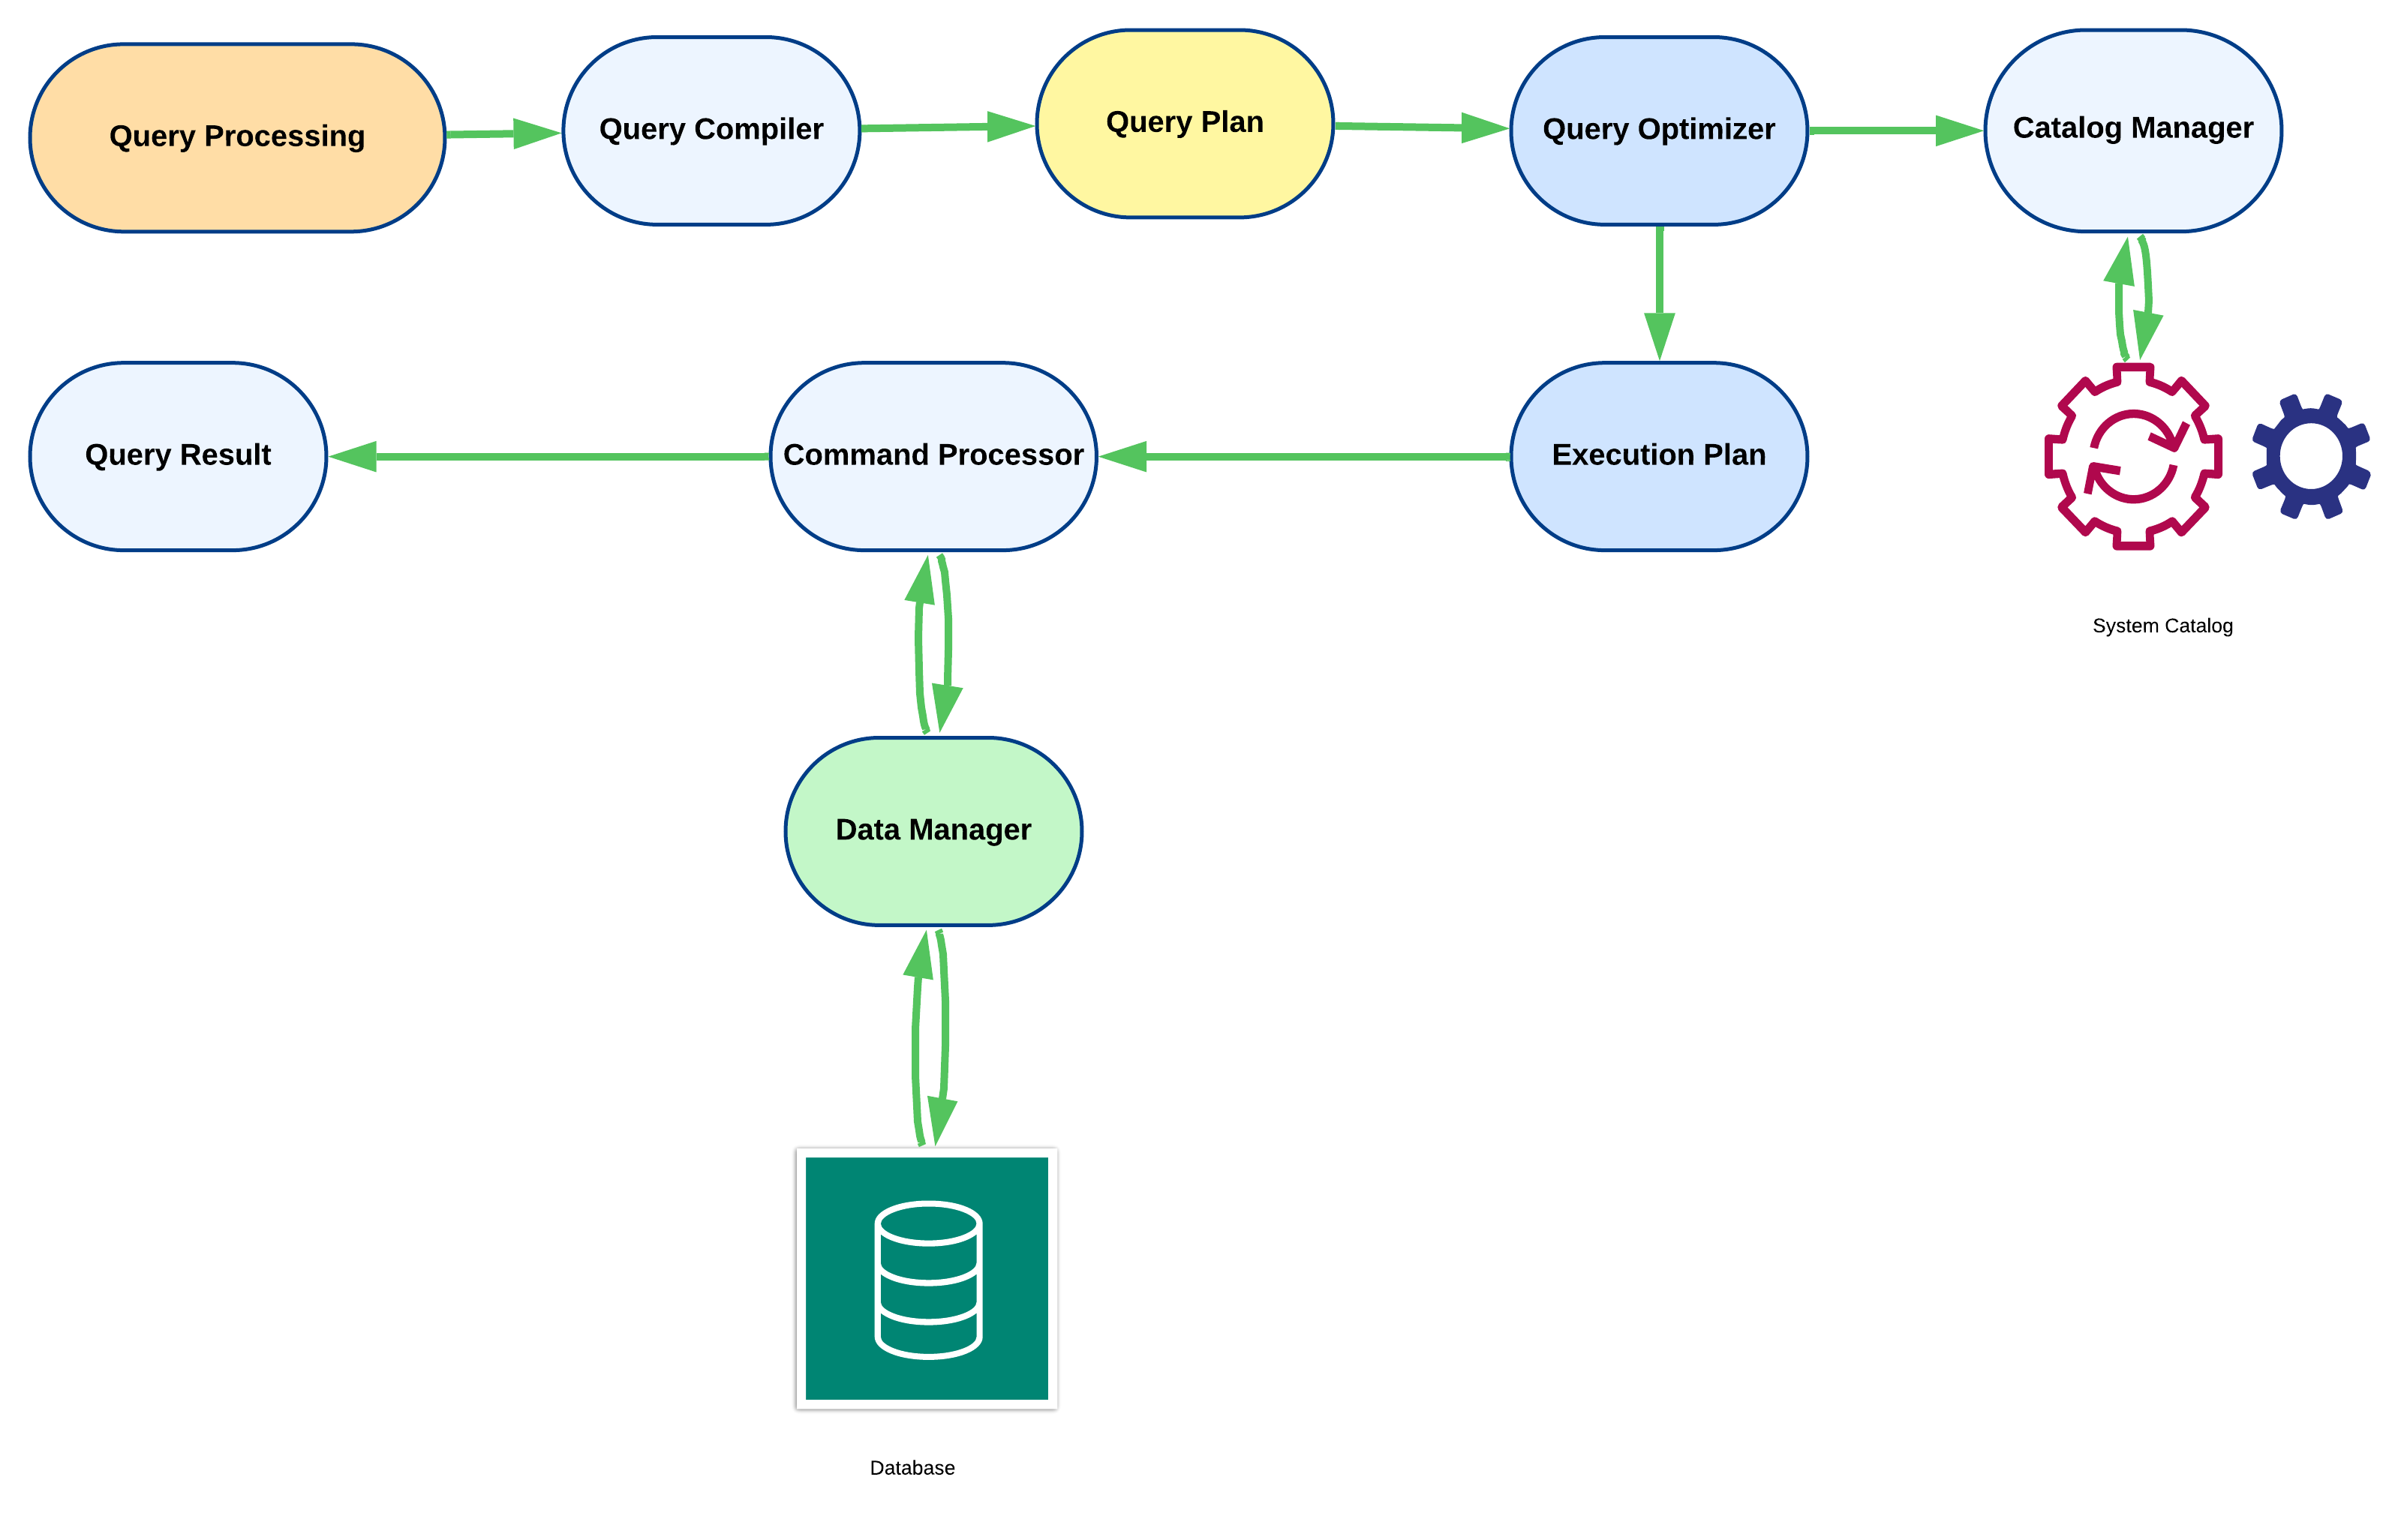
\includegraphics[width=0.5\textwidth]{Figure/Flow of query processing.png}
    \caption[The flow of query processing in DBMS]{The flow of query processing in DBMS ~\cite{wwwnaukricom-no-date} }
     
    \label{fig:my_image} 
\end{figure}
\begin{enumerate}
\item \textbf{Parser:} Query parsing is the first step in query processing. In this step, the database analyzes and breaks down SQL queries by checking syntax and semantics before it is executed by the database engine\cite{wwwnaukricom-no-date}.

    \begin{enumerate}
        \item \textbf{Syntax check:} Syntax validation is the process of validating the structure and format of a query to ensure its functionality and adherence to the SQL language rules before executing it. Here is a general example of a syntax error.
        % Define colors
\definecolor{codegreen}{rgb}{0,0.6,0}  % Green for comments
\definecolor{codegray}{rgb}{0.5,0.5,0.5}  % Gray for numbers
\definecolor{codepurple}{rgb}{0.58,0,0.82}  % Purple for strings
\definecolor{backcolour}{rgb}{0.95,0.95,0.92}  % Light gray background
\definecolor{bordercolor}{rgb}{0.7,0.7,0.7}  % Left border color (gray)
\definecolor{codeblue}{rgb}{0,0,0.8}  % Blue for SQL keywords

\lstdefinelanguage{MySQL}{
    keywords={SELECT, FROM, WHERE, JOIN, ON, INNER, OUTER, LEFT, RIGHT, FULL, GROUP, BY, ORDER, ASC, DESC, AS, COUNT, SUM, AVG, MAX, MIN, DISTINCT, INSERT, INTO, VALUES, UPDATE, SET, DELETE, CREATE, TABLE, PRIMARY, FOREIGN, KEY, DEFAULT, NULL, NOT, CHECK, CONSTRAINT, INDEX, VIEW, MATERIALIZED, PROCEDURE, FUNCTION, TRIGGER, DATABASE, ALTER, DROP, EXEC, IF, EXISTS, UNION, ALL, CASE, WHEN, THEN, ELSE, END, CAST, CONVERT, LIKE, IN, BETWEEN, AND, OR, HAVING, LIMIT, OFFSET},
    sensitive=false,
    morestring=[b]',  % String in single quotes
    morestring=[b]"   % String in double quotes
}
\captionsetup[lstlisting]{font=small}
\lstdefinestyle{sqlstyle}{
    backgroundcolor=\color{backcolour},   
    commentstyle=\color{codegreen},  % Comments in green
    keywordstyle=\bfseries\color{codeblue},  % ✅ SQL Keywords in Blue & Bold
    numberstyle=\scriptsize\color{codegray},  % Row numbers in gray
    stringstyle=\color{codepurple},  % Strings in purple
    basicstyle=\ttfamily\footnotesize,
    breaklines=true,
    captionpos=b,
    numbers=left,      % ✅ Enables row numbers on the left
    stepnumber=1,      % ✅ Row numbers increment by 1
    firstnumber=1,     % ✅ Starts numbering at 1
    numbersep=8pt,     % ✅ Increases space between numbers and SQL code
    xleftmargin=3em,   % ✅ Ensures space inside the left border
    frame=single,      % ✅ Keeps a single border (left-aligned)
    framesep=5pt,      % ✅ Ensures space inside the frame
    rulesepcolor=\color{bordercolor},  % ✅ Matches row numbers with left border
    rulecolor=\color{bordercolor},  % ✅ Sets left border color
    language=MySQL  % ✅ Uses SQL keyword highlighting
}



\begin{lstlisting}[style=sqlstyle, caption={SQL query to check syntax}]
SQL>SELECT * form employees;SELECT * form employees * error at line 1:
FROM   keyword NOT found
WHERE  expected
\end{lstlisting}
        
          Here, the error of the wrong spelling of FROM is given by this check.\vspace{.4cm}
          
        \item \textbf{Semantic check:} It checks whether the statement is meaningful or not. Example: Query contains a table name which does not exist.
        
        
\definecolor{dkgreen}{rgb}{0,0.6,0}
\definecolor{gray}{rgb}{0.5,0.5,0.5}
\definecolor{mauve}{rgb}{0.58,0,0.82}
\lstset{language=SQL,
  basicstyle={\small\ttfamily},
  belowskip=3mm,
  breakatwhitespace=true,
  breaklines=true,
  classoffset=0,
  columns=flexible,
  commentstyle=\color{dkgreen},
  framexleftmargin=0.25em,
  frameshape={}{yy}{}{}, %To remove to vertical lines on left, set `frameshape={}{}{}{}`
  keywordstyle=\color{blue},
  numbers=none, %If you want line numbers, set `numbers=left`
  numberstyle=\tiny\color{gray},
  showstringspaces=false,
  stringstyle=\color{mauve},
  tabsize=3,
  xleftmargin =1em
}
         \begin{lstlisting}
         SQL> SELECT * FROM nonexistent_table;
         SELECT * FROM nonexistent_table
              *
        ERROR at line 1:
        ORA-00942: table or view does not exist
        FROM keyword not found where expected
        \end{lstlisting}
        
        A syntactically correct statement can fail a semantic check, as shown in the above example of a query of a nonexistent table \cite{Oracle}.\vspace{.4cm}
        
        \item \textbf{Shared pool check:} During the parse, the database performs a shared pool check to determine whether it can skip (hash code)\footnote{The hashCode() method is used to generate the hash values of objects.} resource-intensive steps of statement processing. Every query possesses a hash code.\vspace{.4cm}
        
        % Define colors
\definecolor{codegreen}{rgb}{0,0.6,0}  % Green for comments
\definecolor{codegray}{rgb}{0.5,0.5,0.5}  % Gray for numbers
\definecolor{codepurple}{rgb}{0.58,0,0.82}  % Purple for strings
\definecolor{backcolour}{rgb}{0.95,0.95,0.92}  % Light gray background
\definecolor{bordercolor}{rgb}{0.7,0.7,0.7}  % Left border color (gray)
\definecolor{codeblue}{rgb}{0,0,0.8}  % Blue for SQL keywords

\lstdefinelanguage{MySQL}{
    keywords={SELECT, FROM, WHERE, JOIN, ON, INNER, OUTER, LEFT, RIGHT, FULL, GROUP, BY, ORDER, ASC, DESC, AS, COUNT, SUM, AVG, MAX, MIN, DISTINCT, INSERT, INTO, VALUES, UPDATE, SET, DELETE, CREATE, TABLE, PRIMARY, FOREIGN, KEY, DEFAULT, NULL, NOT, CHECK, CONSTRAINT, INDEX, VIEW, MATERIALIZED, PROCEDURE, FUNCTION, TRIGGER, DATABASE, ALTER, DROP, EXEC, IF, EXISTS, UNION, ALL, CASE, WHEN, THEN, ELSE, END, CAST, CONVERT, LIKE, IN, BETWEEN, AND, OR, HAVING, LIMIT, OFFSET},
    sensitive=false,
    morestring=[b]',  % String in single quotes
    morestring=[b]"   % String in double quotes
}

\lstdefinestyle{sqlstyle}{
    backgroundcolor=\color{backcolour},   
    commentstyle=\color{codegreen},  % Comments in green
    keywordstyle=\bfseries\color{codeblue},  % ✅ SQL Keywords in Blue & Bold
    numberstyle=\scriptsize\color{codegray},  % Row numbers in gray
    stringstyle=\color{codepurple},  % Strings in purple
    basicstyle=\ttfamily\footnotesize,
    breaklines=true,
    captionpos=b,
    numbers=left,      % ✅ Enables row numbers on the left
    stepnumber=1,      % ✅ Row numbers increment by 1
    firstnumber=1,     % ✅ Starts numbering at 1
    numbersep=8pt,     % ✅ Increases space between numbers and SQL code
    xleftmargin=3em,   % ✅ Ensures space inside the left border
    frame=single,      % ✅ Keeps a single border (left-aligned)
    framesep=5pt,      % ✅ Ensures space inside the frame
    rulesepcolor=\color{bordercolor},  % ✅ Matches row numbers with left border
    rulecolor=\color{bordercolor},  % ✅ Sets left border color
    language=MySQL  % ✅ Uses SQL keyword highlighting
}



\begin{lstlisting}[style=sqlstyle, caption={SQL query to check shared pool}]
     ALTER SESSION SET OPTIMIZER_MODE=ALL_ROWS;
     ALTER SYSTEM FLUSH SHARED_POOL; 
     SELECT * FROM Employees WHERE DepartmentID = 10;

\end{lstlisting}
        
        In this example, When the \textbf{SELECT} statement is executed, the SQL server checks the plan cache to see if an execution plan for this identical query already exists. If a matching execution plan is found in the cache\footnote{A cache in SQL is a high-speed data storage layer that temporarily stores frequently accessed data to improve query performance and reduce database load} (a ``cache hit''), SQL server reuses it, allowing for quicker execution without going through the parsing and optimization steps again.
        
    \end{enumerate}
    
%\begin{figure}[h]
   % \centering
   % 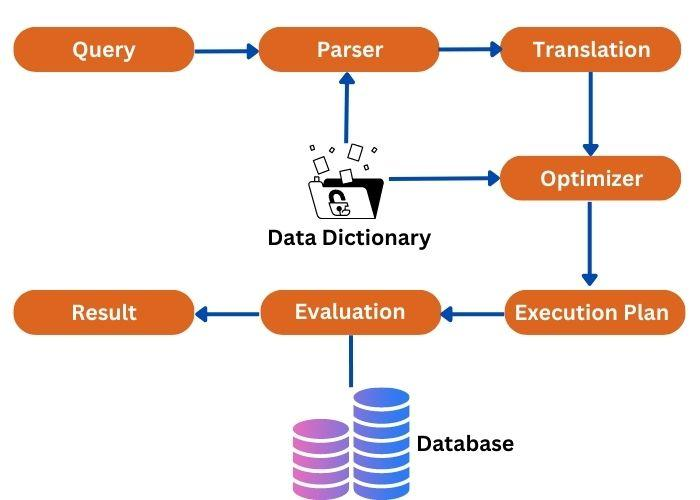
\includegraphics[width=0.5\textwidth]{Figure/Query processing.jpg}
   % \caption[The flow of query processing in DBMS]{The flow of query processing in DBMS \cite{Oracle}}
    %\label{fig:my_image}
%\end{figure}
    
    \item \textbf{Optimizer}: After parsing the query, the DBMS starts to find the most efficient way of executing the provided query. The factors for the query follow some optimization process. During the optimization stage, at least one complex parsing of one unique DML\footnote{DML  (data manipulation language) refers to a computer programming language that allows you to add (insert), delete (delete), and alter (update) data in a database.} statement must be done. The database never optimizes DDL\footnote{Data definition or data description language (DDL) is a syntax for creating and modifying database objects such as tables, indices, and users.} unless it includes a DML component, such as a sub-query, which needs optimization. Such operations are used for selecting data, inserting something, and updating. After everything is completed, then the evaluation step is made. In this step, the DBMS returns the result.
    
    \item \textbf{Result:} After getting the best execution plan, the DBMS starts the execution of the optimized query and operates on data, including selecting the data, inserting something, and updating the data. Once everything is completed, DBMS returns the result after the evaluation step \cite{Query,QueryProcessing,Oracle}.
    
\end{enumerate}

\subsection{Query Optimization } Code is written with the goal of optimal logic in terms of both space and time complexity. Likewise, when database queries are written, they are desired to be optimal in terms of their execution time and resource utilization. Query optimization is a crucial aspect of DBMS that seeks the most efficient way to execute a given query by considering a variety of query execution strategies. It minimizes the total cost or the total response time for the execution of a query. It is one of the key factors that affect the application performance.\vspace{.4cm}

The result of a query is generated by processing the rows and columns in a database in a way that yields the requested information. Since database structures are complex, in most cases, and especially for not very simple queries, the needed data for a query can be collected from a database by accessing it in different ways through different data structures and in different orders \cite{selinger-1979}. Each different method usually requires varying processing times. The time it takes to process the same query can vary significantly, ranging from a fraction of a second to hours, depending on the selected method. The goal of query optimization is to determine how to process a given query in the shortest time possible. The significant potential variance in processing time justifies the need for query optimization. However, identifying the exact optimal query plan from all available options is often very complex, time-consuming, and frequently impractical. Therefore, query optimization generally aims to approximate the optimum by evaluating several reasonable alternatives to deliver results within an acceptable time frame. \vspace{.4cm}

There is a trade-off between the amount of time spent figuring out the best query plan and the quality of the choice, and the optimizer may not choose the best answer on its own. Database management systems have different qualities and ways of balancing these two. Cost-based query optimizes and evaluates the resource footprints of various query plans and uses this as the basis for plan selection. These assign an estimated cost to each possible query plan and choose the plan with the smallest cost. Cost is used to estimate the runtime cost of evaluating the query in terms of the number of I/O operations required, CPU path length, amount of disk buffer space, disk storage service time, and connection consumption between units of parallelism, and other factors identified from the data directory. The set of query strategies is formed by examining the possible access paths, e.g., primary index, secondary index access, full file scan, and various relational table join techniques, e.g., Merge join, has join, and Product join. The search space can become quite large depending on the complexity of the SQL query. There are two types of optimization. These consist of logical optimization, which generates a sequence of relational algebra to solve the query, and physical optimization, which is used to determine the means of carrying out each operation \cite{dremio-2024}.\vspace{.4cm}

Query optimization is crucial for databases to enhance efficiency and performance. It enables organizations to significantly increase query speed, decrease data retrieval times, and minimize resource usage. By doing this, it not only identifies and addresses issues like slow queries and bottlenecks but also ensures that the database operates at its best, delivering faster and more reliable data processing. Ultimately, effective optimization results in a better user experience and heightened productivity throughout the organization\cite{team-2023, r-2024}.


\subsubsection{Database Query Performance Metrics}
The following metrics play a vital role in effectively measuring the performance of SQL queries. However, most relevant metrics may vary depending on the specific database system and application requirements.
Here is a summary of key metrics used to evaluate and enhance query performance \cite{chwesewicz-2024}.
\begin{itemize}
    \item\textbf{Query execution time}: Query execution time refers to the duration it takes for a database to process and return results for a given SQL query. Measured in seconds or milliseconds. Lower execution time indicates better performance.
    \item\textbf{Query throughput}: It measures the number of queries or operations a database can handle per unit of time, typically expressed as transactions per second (TPS) and queries per second(QPS).
    \item\textbf{Resource utilization}: Measures the percentage of time the CPU is occupied processing database operations. High CPU or memory usage can indicate a heavy processing load or un-optimized queries.
\end{itemize}

\subsubsection{Key Optimization Techniques:}

Optimizing a query is critical for increasing database performance. There are various optimization strategies. However, the following are the most widely used:

 \begin{itemize}
     \item \textbf{Indexing}: Indexing is a crucial technique for query optimization in databases. It's named indexing because of how an index works in a book. An index is a structure that holds the field the index is sorting and a pointer from each record to their corresponding record in the original table where data is actually stored \cite{tomar-2021,atlassian-no-date}.
     \item \textbf{Query rewriting}: It is a technique used in query optimization to transform a given database query into an equivalent form that executes more efficiently. It is one of the initial phases of query processing, where the original query is parsed and translated into an internal representation. This method is particularly useful for complex queries, including those queries that have many sub-queries or many join \cite{pitoura-2009,unknown-IBM-25-2024}.
     
     \item \textbf{Partitioning}: This optimization method is especially effective for large databases. It involves splitting a large table or index into smaller segments to make the query more manageable pieces. Each partition acts as a separate entity that can be managed independently \cite{planck-2024}.
     
     \item \textbf{Caching:} It is a vital technique that involves storing cache results in RAM\footnote{ RAM is a form of electronic computer memory that can be read and changed in any order, typically used to store working data and machine code.} for ultra-fast access or on disk of frequently executed queries. This is particularly useful for queries that are executed across multiple requests \cite{Bit-Fetch-2024}.
     
     \item\textbf{Materialized view}: Materialized views are a powerful tool for query optimization. This paper has demonstrated the significant impact of materialized views on query optimization, highlighting their role as a crucial tool for improving database performance. A detailed explanation can be found in the \hyperref[term:materialized_views]{chapter 2.6}.\vspace{.4cm}
     
 \end{itemize}
 
 \subsection{Reasons for Using Materialized View for Query Optimization}
 Materialized views(MVs) offer several compelling reasons for query optimization in a scheduled manner without compromising accuracy or freshness. Here are some key points:
 
\begin{itemize}
    \item\textbf{Precomputed result:} Materialized views store the results of a query that allows subsequent queries to access these precomputed results directly rather than recalculating them from the base tables. These results are updated periodically or on-demand based on the underlying data changes \cite{khan-2023,Risingwave-no-date}.
    
    \item\textbf{Reduced Query complexity:} The main reason for creating materialized views is to improve query performance. It stores a snapshot of the data, which reduces the need for intricate query design, as we get the accesses precomputed results directly \cite{Risingwave-no-date,Databricks-no-date}.
    
    \item\textbf{Efficient use of resources:} As we get the data from pre-computed data and do not need to run a full query every time materialized views decrease the computational load on database servers. It leads to faster query response time, improved overall system performance, and requires fewer resources \cite{google-no-date, khan-2023}.
    
\end{itemize}\vspace{.4cm}

The motivation for using materialized views is to enhance performance. However, the additional effort involved in managing them can become a significant concern for system administration. Common management tasks for materialized views include identifying which views to generate, indexing them, and ensuring that all materialized views and indexes are refreshed properly whenever the database is updated. Standard management activities also involve reviewing which materialized views have been used and evaluating how effectively each view has impacted workload performance. It's also important to determine how much space materialized views occupy and which views should be removed. Outdated information should be archived, and materialized view data that is no longer useful should be deleted \cite{Ashadevi2008CostEA,1363763}.

\subsubsection{Challenges in Query Optimization} Query optimization is a crucial aspect of database management, aiming to improve the performance and efficiency of SQL queries. Opta data group, a company specializing in healthcare data management, faces several challenges with query optimization in its MSSQL environment. Given the vast amount of patient and operational data they handle, inefficient queries can lead to slow response times and increased resource consumption \cite{Flipico-2024}. The following example scenario shows query challenges:\vspace{.4cm}


% Define colors
\definecolor{codegreen}{rgb}{0,0.6,0}  % Green for comments
\definecolor{codegray}{rgb}{0.5,0.5,0.5}  % Gray for numbers
\definecolor{codepurple}{rgb}{0.58,0,0.82}  % Purple for strings
\definecolor{backcolour}{rgb}{0.95,0.95,0.92}  % Light gray background
\definecolor{bordercolor}{rgb}{0.7,0.7,0.7}  % Left border color (gray)
\definecolor{codeblue}{rgb}{0,0,0.8}  % Blue for SQL keywords

\lstdefinelanguage{MySQL}{
    keywords={SELECT, FROM, WHERE, JOIN, ON, INNER, OUTER, LEFT, RIGHT, FULL, GROUP, BY, ORDER, ASC, DESC, AS, COUNT, SUM, AVG, MAX, MIN, DISTINCT, INSERT, INTO, VALUES, UPDATE, SET, DELETE, CREATE, TABLE, PRIMARY, FOREIGN, KEY, DEFAULT, NULL, NOT, CHECK, CONSTRAINT, INDEX, VIEW, MATERIALIZED, PROCEDURE, FUNCTION, TRIGGER, DATABASE, ALTER, DROP, EXEC, IF, EXISTS, UNION, ALL, CASE, WHEN, THEN, ELSE, END, CAST, CONVERT, LIKE, IN, BETWEEN, AND, OR, HAVING, LIMIT, OFFSET},
    sensitive=false,
    morestring=[b]',  % String in single quotes
    morestring=[b]"   % String in double quotes
}

\lstdefinestyle{sqlstyle}{
    backgroundcolor=\color{backcolour},   
    commentstyle=\color{codegreen},  % Comments in green
    keywordstyle=\bfseries\color{codeblue},  % ✅ SQL Keywords in Blue & Bold
    numberstyle=\scriptsize\color{codegray},  % Row numbers in gray
    stringstyle=\color{codepurple},  % Strings in purple
    basicstyle=\ttfamily\footnotesize,
    breaklines=true,
    captionpos=b,
    numbers=left,      % ✅ Enables row numbers on the left
    stepnumber=1,      % ✅ Row numbers increment by 1
    firstnumber=1,     % ✅ Starts numbering at 1
    numbersep=8pt,     % ✅ Increases space between numbers and SQL code
    xleftmargin=3em,   % ✅ Ensures space inside the left border
    frame=single,      % ✅ Keeps a single border (left-aligned)
    framesep=5pt,      % ✅ Ensures space inside the frame
    rulesepcolor=\color{bordercolor},  % ✅ Matches row numbers with left border
    rulecolor=\color{bordercolor},  % ✅ Sets left border color
    language=MySQL  % ✅ Uses SQL keyword highlighting
}

\begin{lstlisting}[style=sqlstyle, caption={Challenges in query optimization}]
SELECT *
FROM   patients
       JOIN treatments
         ON patients.patientid = treatments.patientid
WHERE  treatmentdate >= '2024-12-02'; 
\end{lstlisting}


The join condition in the above query relates the two tables, namely `` Patients '' and `` Treatment ''. Suppose the `` PatientID '' column in both the ``Patients'' and `` Treatment'' tables is not indexed properly. In that case, the database may perform a full table scan, and that might happen when only a few columns are required from a very big table, and this would cause very slow response times and a lot of resources consumed. Further details about the key challenges during query optimization are discussed below:

\begin{itemize}
    \item\textbf{Data Fragmentation and Localization}: Dealing with how data is partitioned and distributed across multiple nodes. Data can be fragmented both horizontally and vertically and spread across nodes. Balancing between local execution and data transfer is also challenging. 
    \item\textbf{Query Decomposition and Allocation}: It refers to the process of breaking down a query into sub-queries and assigning them to different nodes. It is challenging to choose the best sub-queries and nodes.
    \item\textbf{Complexity of Query Execution Plans}: Query optimization involves various techniques. Mastering these techniques can be challenging in finding the most efficient one, especially for complex or multi-table queries.
    \item\textbf{Dependency on Indexes}: Proper indexing improves query performance, but failing to create or maintain supporting indexes can result in inefficient query executions. Managing and updating indexes as data grows and changes can become a challenge Expressed during optimization as a cost function. The common choice is to minimize response time within given resource limitations.\cite{team-2020,etutorials-03-2024,editor-ijmter-2015}.
\end{itemize}

During the experiment, there were numerous challenges encountered, as mentioned above. It was challenging to split materialized views across multiple nodes and minimize data transfer costs due to data fragmentation. It was not straightforward to divide queries into sub-queries and split them into nodes to get the best execution efficiency. Query execution plans were complicated with joins between multiple tables and aggregations, and it was challenging to decide the best way to execute them. In addition, proper indexing was necessary to maintain query performance since the absence of creating or updating indexes resulted in inefficient execution. The PSO algorithm avoids all these complexities since it minimizes the cost function to obtain minimum response time and resource consumption. 

\subsubsection*{Optimization Goals:}

\begin{itemize}
    \item Minimize response time
    \item Minimize resource consumption
    \item Minimize time to the first tuple
    \item Maximize throughput
\end{itemize}\vspace{.4cm}

This paper shares the same optimization goals, particularly focusing on minimizing response time. The primary objective is to enhance query performance by limiting execution latency and minimizing resource consumption and time to the first tuple. Maximizing throughput is also considered to enable efficient handling of multiple queries. By using materialized views and the PSO algorithm, this work aims to accomplish all these goals, with an emphasis on optimizing response time to improve query execution more quickly.



\subsection{What is a View in SQL:}
A view in SQL is a virtual table that is generated by an SQL query. It does not store data physically but retrieves it from the underlying base table. Views are compiled at runtime, and they simplify the presentation of data from one or more tables without modifying the original data. It can be made over one or more database tables. Generally, those columns that need to be queried repeatedly are put into a view. Once the view is created, an index can be made, the view can be triggered, and the view can be queried as a table. The view can function as a filter for specific tables it references \cite{chauhan-2024, Rohan_Vats-2024}.\vspace{.4cm}

A view is a component of a database that provides a specific user with an impression of data while restricting access to the original database tables. In this context, the original tables are known as view tables. A view can represent data from a database, facilitate a specific selection of data, or compute new data that reflects the contents of the underlying base tables. In other words, every analytical operation derived from the base table data originates from a view table.\vspace{.4cm}




The following example explains the concept of view:


\definecolor{dkgreen}{rgb}{0,0.6,0}
\definecolor{gray}{rgb}{0.5,0.5,0.5}
\definecolor{mauve}{rgb}{0.58,0,0.82}
\lstset{language=SQL,
  basicstyle={\small\ttfamily},
  belowskip=3mm,
  breakatwhitespace=true,
  breaklines=true,
  classoffset=0,
  columns=flexible,
  commentstyle=\color{dkgreen},
  framexleftmargin=0.25em,
  frameshape={}{yy}{}{}, %To remove to vertical lines on left, set `frameshape={}{}{}{}`
  keywordstyle=\color{blue},
  numbers=none, %If you want line numbers, set `numbers=left`
  numberstyle=\tiny\color{gray},
  showstringspaces=false,
  stringstyle=\color{mauve},
  tabsize=3,
  xleftmargin =1em
}
         \begin{lstlisting}
CREATE VIEW AokCustommers AS
SELECT CustomerName
FROM Customers
WHERE Country = 'Germany';
        \end{lstlisting}

 In this example, the view ``AokCustomers'' is created to simplify access to customer names, specially from Germany. This view dynamically retrieves the relevant data from the ``Customers'' table, allowing for easier and more efficient data retrieval.
 
\subsubsection{Types of Views:}

There are two types of view in SQL server
\begin{itemize}
    \item \textbf{System defined view}: The system-defined views are predefined views that already exist in the master database of the SQL server, such as tempdb, master, and temp. Each of the databases has its properties and functions. These system views will be automatically attached to any user-defined database. It will expose the metadata of the database, and it can be used to get all possible information about the instance of the SQL server or database objects, columns, and contains. There are three types of System-defined views: Information Schema, Catalog View, and Dynamic Management View \cite{chauhan-2024}.
    \item \textbf{User-defined view}: These are the types of views that the user created to meet their specific requirements. It can also be divided into three types: simple, complex, and materialized views that help to organize, secure, and simplify access to database information \cite{javapoint-author-2024}.
\end{itemize}
   
\subsection{Materialized Views}\label{term:materialized_views}
\noindent\textit{Materialized views, also known as materialized tables or summary tables, are database objects that physically store the result of a query. Unlike regular views, which are virtual and compute their results on the fly, materialized views pre-compute and store the query results, allowing for faster retrieval and improved query performance.} \vspace{.3cm}

Materialized views in databases optimize query performance by pre-computing and storing the results of complex queries involving aggregations and joins. This reduces the computational load during execution, significantly speeding up response times.\vspace{.4cm}

 A special type of view is materialized views. It refers to the fact that the contents of the view are stored in the form of a separate table in the database system. MV is designed to the user's requirements. An MV definition includes aggregation functions like MIN\footnote{The MIN function returns the smallest value in a set of non-NULL values.}, MAX\footnote{The MAX function returns the largest value in a set of non-NULL values.}, COUNT(DISTINCT), COUNT(*)\footnote{COUNT returns the number of rows that match the specified criteria.}, SUM\footnote{SUM calculates the total of a set of values.}, and AVG\footnote{AVG computes the average value of a set of non-NULL values.}, one or more tables joined together, and a GROUP BY operation on attributed and basic data definition language operation such as CREATE; ALTER and DROP may be applied on tables \cite{Kardel_Thakare}. MV is a decision support/ data warehousing system tool that can increase the speed of queries that access a large number of records by many orders of magnitude \cite{Kishan_Sainath_no_date}. Nevertheless, materialized views can also be stored as a file or a data structure in memory. In addition to that, a virtual view would be loaded from the base table when requested. While the on-demand idea behind virtual views is certainly desirable \cite{jan-no-date,ashadevi-2024}.\vspace{.4cm}



A materialized view (sometimes called a sorted, projected and materialized view or SPM view) is a view whose columns have been sorted, projected and materialized.\cite{IBM} In database systems, optimize query performance by pr-computing and storing the result of complex queries involving aggregations and joins. As they store the results physically in a table, re-computation of a query is not needed again. When the view is already materialized at any time, the same query is entered into the system. This reduces the computational load during the execution, significantly speeding up the response times.\vspace{.4cm}

\subsubsection{Working Principle of Materialized Views}
The working principle of MV can be described as follows:

\begin{itemize}
    \item\textbf{Pre-computations:} It stores the results of queries that involve complex join and aggregations. These results are pre-computed and stored in the database, reducing the time needed to fetch the data when required.
    \item\textbf{Storage and retrieval:} The data in a materialized view is periodically refreshed to reflect changes in the underlying tables. The refresh can be scheduled or triggered by specific events, depending on the use case and requirements.
    \item\textbf{Refresh mechanism:}  Materialized views need to be refreshed to stay up to date with the underlying data.\vspace{.4cm}

    \begin{itemize}
        \item\textbf{Full Refresh:} The entire view is recomputed from scratch.
        \item\textbf{Incremental Refresh:} Only the changes since the last refresh are applied.
        \item\textbf{On Demand Refresh:} Triggered by specific events or user requests.
    \end{itemize}
 
\end{itemize}\vspace{.4cm}

Materialized views must be refreshed every now and then to maintain synchrony with the base information. This research employs the on-demand refresh mechanism among several strategies used. The on-demand refresh strategy updates the materialized view when specific events or user requests happen. The on-demand refresh strategy is employed in this research due to its flexibility and ability to save resources while allowing targeted updates when precision in data is critical.

\subsubsection{Types of Materialized Views}
The most prevalent forms of materialized views in database management systems are:

\vspace{.4cm}

\begin{enumerate}[label=\alph*)]
 \item\textbf{ Materialized views with aggregates:} Materialized views with aggregates store the results of queries that perform aggregate calculations (e.g., SUM, COUNT, AVG, MIN, MAX) over large datasets. These views are particularly useful for optimizing query performance in scenarios that involve complex aggregations over vast amounts of data, such as reporting, analytics, and decision support systems. The explanation is demonstrated with the following example:\vspace{.4cm}
    
    
\definecolor{dkgreen}{rgb}{0,0.6,0}
\definecolor{gray}{rgb}{0.5,0.5,0.5}
\definecolor{mauve}{rgb}{0.58,0,0.82}
\lstset{language=SQL,
  basicstyle={\small\ttfamily},
  belowskip=3mm,
  breakatwhitespace=true,
  breaklines=true,
  classoffset=0,
  columns=flexible,
  commentstyle=\color{dkgreen},
  framexleftmargin=0.25em,
  frameshape={}{yy}{}{}, %To remove to vertical lines on left, set `frameshape={}{}{}{}`
  keywordstyle=\color{blue},
  numbers=none, %If you want line numbers, set `numbers=left`
  numberstyle=\tiny\color{gray},
  showstringspaces=false,
  stringstyle=\color{mauve},
  tabsize=3,
  xleftmargin =1em
}
         \begin{lstlisting}
 
CREATE MATERIALIZED VIEW SalesSummary
AS
SELECT
    ProductID,
    Region,
    CategoryID,
    SUM(SalesAmount) AS TotalSales,
    AVG(SalesAmount) AS AvgSales,
    COUNT(*) AS NumberOfSales
FROM Sales
GROUP BY ProductID, Region, CategoryID;

        \end{lstlisting}

    In this example, the materialized view ``salesSummary'' precomputes the SUM, AVG, and COUNT for sales data grouped by ProductID, Region, and CategoryID.

    \item\textbf{Materialized views with join }: Materialized views with joins store the results of queries that involve multiple tables combined using join operations (e.g., INNER JOIN, LEFT JOIN, RIGHT JOIN). These types of materialized views can significantly speed up complex queries that frequently access multiple related tables. By precomputing the join results, the materialized view avoids the need to recompute them during every query execution. The explanation is made clear with the following example: \vspace{.4cm}
    
    
\definecolor{dkgreen}{rgb}{0,0.6,0}
\definecolor{gray}{rgb}{0.5,0.5,0.5}
\definecolor{mauve}{rgb}{0.58,0,0.82}
\lstset{language=SQL,
  basicstyle={\small\ttfamily},
  belowskip=3mm,
  breakatwhitespace=true,
  breaklines=true,
  classoffset=0,
  columns=flexible,
  commentstyle=\color{dkgreen},
  framexleftmargin=0.25em,
  frameshape={}{yy}{}{}, %To remove to vertical lines on left, set `frameshape={}{}{}{}`
  keywordstyle=\color{blue},
  numbers=none, %If you want line numbers, set `numbers=left`
  numberstyle=\tiny\color{gray},
  showstringspaces=false,
  stringstyle=\color{mauve},
  tabsize=3,
  xleftmargin =1em
}
         \begin{lstlisting}
CREATE MATERIALIZED VIEW CustomerOrderSummary
AS
SELECT
    c.CustomerID,
    c.CustomerName,
    o.OrderID,
    o.OrderDate,
    p.ProductID,
    p.ProductName,
    o.Quantity,
    o.TotalAmount
FROM
    Customers c
JOIN
    Orders o ON c.CustomerID = o.CustomerID
JOIN
    Products p ON o.ProductID = p.ProductID;

        \end{lstlisting}

    In this example, the materialized view ``CustomerOrderSummary''
    stores the results of the joins between the customers, orders and products table.
    
    \item \textbf{Hybrid materialized views}: Hybrid materialized views combine features of both aggregates and join-based materialized views, optimizing performance for queries that require both aggregations and joins between multiple tables. They are designed to handle more complex queries efficiently, as they store pre-computed results that involve both aggregated data and joined tables. Hybrid materialized views are particularly useful in environments like data warehouses or reporting systems where queries often need to summarize and relate data from various sources. \vspace{.4cm}
    
    \definecolor{codegreen}{rgb}{0,0.6,0}  % Green for comments
\definecolor{codegray}{rgb}{0.5,0.5,0.5}  % Gray for numbers
\definecolor{codepurple}{rgb}{0.58,0,0.82}  % Purple for strings
\definecolor{backcolour}{rgb}{0.95,0.95,0.92}  % Light gray background
\definecolor{bordercolor}{rgb}{0.7,0.7,0.7}  % Left border color (gray)
\definecolor{codeblue}{rgb}{0,0,0.8}  % Blue for SQL keywords

\lstdefinelanguage{MySQL}{
    keywords={SELECT, FROM, WHERE, JOIN, ON, INNER, OUTER, LEFT, RIGHT, FULL, GROUP, BY, ORDER, ASC, DESC, AS, COUNT, SUM, AVG, MAX, MIN, DISTINCT, INSERT, INTO, VALUES, UPDATE, SET, DELETE, CREATE, TABLE, PRIMARY, FOREIGN, KEY, DEFAULT, NULL, NOT, CHECK, CONSTRAINT, INDEX, VIEW, MATERIALIZED, PROCEDURE, FUNCTION, TRIGGER, DATABASE, ALTER, DROP, EXEC, IF, EXISTS, UNION, ALL, CASE, WHEN, THEN, ELSE, END, CAST, CONVERT, LIKE, IN, BETWEEN, AND, OR, HAVING, LIMIT, OFFSET},
    sensitive=false,
    morestring=[b]',  % String in single quotes
    morestring=[b]"   % String in double quotes
}

\lstdefinestyle{sqlstyle}{
    backgroundcolor=\color{backcolour},   
    commentstyle=\color{codegreen},  % Comments in green
    keywordstyle=\bfseries\color{codeblue},  % ✅ SQL Keywords in Blue & Bold
    numberstyle=\scriptsize\color{codegray},  % Row numbers in gray
    stringstyle=\color{codepurple},  % Strings in purple
    basicstyle=\ttfamily\footnotesize,
    breaklines=true,
    captionpos=b,
    numbers=left,      % ✅ Enables row numbers on the left
    stepnumber=1,      % ✅ Row numbers increment by 1
    firstnumber=1,     % ✅ Starts numbering at 1
    numbersep=8pt,     % ✅ Increases space between numbers and SQL code
    xleftmargin=3em,   % ✅ Ensures space inside the left border
    frame=single,      % ✅ Keeps a single border (left-aligned)
    framesep=5pt,      % ✅ Ensures space inside the frame
    rulesepcolor=\color{bordercolor},  % ✅ Matches row numbers with left border
    rulecolor=\color{bordercolor},  % ✅ Sets left border color
    language=MySQL  % ✅ Uses SQL keyword highlighting
}

\begin{lstlisting}[style=sqlstyle, caption={Hybrid materialized views}]

CREATE materialized VIEW productsalessummary
AS SELECT r.regionname,
          p.categoryid,
          p.productname,
          c.customerid,
          SUM(o.quantity)    AS TotalQuantity,
          SUM(o.totalamount) AS TotalSales
   FROM   customers c
          join orders o
            ON c.customerid = o.customerid
          join products p
            ON o.productid = p.productid
          join regions r
            ON c.regionid = r.regionid
   GROUP  BY r.regionname,
             p.categoryid,
             p.productname,
             c.customerid; 

\end{lstlisting} 
    
This materialized view, ``ProductSalesSummary'' stores precomputed join results between customers, orders, products, and regions, as well as aggregate data on the total quantity and total sales.
    
\end{enumerate}

This paper uses materialized views with aggregates for query optimization using the PSO algorithm. Materialized views with aggregates precompute and store summarized data, such as sums, averages, and counts, which avoids significant query execution time by preventing on-the-fly computations. This method is extremely efficient for analytical query optimization and response time improvement.

Materialized views and hybrid materialized views have not been utilized in this paper because they introduce additional complexity when it comes to maintaining data consistency and require greater storage space. Materialized joins are suitable to be utilized to speed up complex joins but can introduce higher maintenance cost and more data transfer in the distributed system. Hybrid materialized views join and aggregate, but because of their complexity, they are not as well-suited to the performance goals of this research. Aggregated materialized views were therefore chosen for their simplicity and effectiveness in query execution time minimization.

\subsubsection{Materialized View vs Database View:} With the usual syntax of creating a view, we create a database view, which is different from the materialized view because a normal database view is just a virtual table that is defined by a SQL query. It is stored in the user database and can be accessed by users who have appropriate permissions. An MV view does not store any data itself; it is simply a way of presenting data from one or more tables in different ways. Materialized views are disk-based and are updated periodically based on the query definition \cite{Stackoverflow-author-08-2008}. Views are virtual and run the query definition each time they are accessed. Materialized views are useful when data is accessed frequently and updated infrequently.

\subsection{Algorithm Related to the Query Optimization }
Query optimization algorithms are the methods that the database system uses to generate and select the best query execution plan for a given query. Several algorithms are commonly used to address the complex challenge of finding optimal query execution plans, including heuristic-based, cost-based, and rule-based. Heuristic-based uses predefined rules and guidelines to guide the query process, cost-based evaluates multiple execution plans and chooses the one with the lowest estimated cost, while rule-based optimization applies a fixed set of predefined rules to transform queries without considering actual data statistics. In this paper, the focus is on a cost-based algorithm like the particle swarm optimization approach, as it provides more accurate and efficient complex search spaces and converges optimal query plans.

\subsubsection{Particle Swarm Optimization Algorithm}
Particle swarm optimization is a type of optimization algorithm that depends quite on the behavior of natural organisms, such as birds or fish, that move together to achieve a common goal. A group of particles navigates the problem solution space in search of the best possible solution. Each particle adjusts its position in accordance with its best-known solution (personal best)\footnote{$P_Best$ known as local best position among all the particles.} as well as the best solution discovered by the entire group (global best)\footnote{$G_Best$ known as global best position among all the particles.}. This allows particles to converge on ideal solutions across iterations \cite{subhasis-2023}.\vspace{.4cm}

 In the case of query optimization, this makes use of all such aspects in order to optimize the configuration view, index, or query execution plan with minimum query response and resource usage in the database management systems. Here, PSO represents solution(s) as particles, for example, combinations of materialized views, which move through the solution space according to their own experiences and the swarm's experiences. By constantly changing the position of such particles, PSO iteratively finds the best optimal\footnote{Best optimal emphasizes that the solution is not just optimal (i.e., a good solution) but is the best among all possible optimal solutions found during the optimization process.} solution or near-optimum solution that has the best trade-off between query and costs of maintenance and hence becomes a very powerful means for database administrators keen on optimizing very complex database environments. Two main equations are involved in the process of PSO algorithm:\vspace{.4cm}
\begin{itemize}
    \item \textbf{Velocity update:} In this step, each particle in the swarm updates its velocity using the computed values of the individual and global best solutions and its current best position. 

\begin{equation}
v_i(t+1) = W \cdot v_i(t) + c_1 \cdot r_1 \cdot (P_Best_i - x_i(t)) + c_2 \cdot r_2 \cdot (G_Best - x_i(t))
\end{equation}

\textbf{Where:}
\begin{itemize}
    \item \( v_i(t) \): Current velocity of particle \( i \) at time \( t \).
    \item \( W \): Inertia weight that controls the influence of the previous velocity on the current velocity.
    \item \( c_1 \): Cognitive coefficient representing the weight given to the particle's own experience (personal best).
    \item \( r_1 \): A random number uniformly distributed between 0 and 1, introducing stochastic behavior.
    \item \( G_ Best_i \): The personal best position that particle \( i \) has encountered so far.
    \item \( x_i(t) \): Current position of particle \( i \) at time \( t \).
    \item \( c_2 \): Social coefficient representing the weight given to the global best position found by any particle in the swarm.
    \item \( r_2 \): Another random number uniformly distributed between 0 and 1.
    \item \( P_Best \): The global best position found by any particle in the swarm.
\end{itemize}



    The acceleration factor of the c1 and c2 coefficients is related to individual and social aspects. It determines how much confidence a particle has in itself and its neighbors to find an optimal solution \cite{baeldung2024pso}
    
    \item \textbf{Position update:} In this part, a new location of the particle is updated using the newly calculated velocity. This movement allows the particle to explore within the search space based on both its previous position and the velocity defined by its own experience and that of the swarm. The parameters of position and velocity are co-dependent.
    
    
\begin{equation}
x_i(t+1) = x_i(t) + v_i(t+1)
\end{equation}

\textbf{Where:}
\begin{itemize}
    \item \( x_i(t) \): Current position of particle \( i \) at time \( t \).
    \item \( v_i(t+1) \): Updated velocity of particle \( i \) at time \( t+1 \).
    \item \( x_i(t+1) \): New position of particle \( i \) at the next time step.
\end{itemize}

%\textbf{Description:} The position update equation states that the new position of a particle is calculated by adding its updated velocity to its current position. This movement allows the particle to explore the search space based on both its previous position and the velocity determined by its own experience and that of the swarm.



\end{itemize} 

\textbf{Example Scenario:} Consider a scenario where a company has a database with three tables: ``Patients'', ``Treatments'', and ``Billing''. They frequently run a complex query that joins these tables and applies a filter but do not know which materialized views can speed up the query. To solve this problem, they can use the PSO algorithm to determine the best combination. Each particle represents a different combination of potential configurations of materialized views. For example:

 \begin{itemize}
     \item Particle 1: [0,1,0] - Materialized view for total patients by doctor.
     \item Particle 2: [1,0,1] - Materialized view for average billing per treatment type.
     \item Particle 3: [1,1,0] - Materialized view for monthly admission.
 \end{itemize}

Each particle's fitness\footnote{Particle fitness refers to the measure of how well a particular combination of materialized views performs in terms of query execution time and maintenance cost} is evaluated by running the query based on the execution time and maintenance cost. For example:

\begin{itemize}
     \item Particle 1 fitness: 1.5 ms
     \item Particle 2 fitness: 1.3 ms
     \item Particle 3 fitness: 2.1 ms
 \end{itemize}
 
 To determine $G_{\text{Best}}$, the algorithm starts by initializing each particle position and evaluating its fitness. The particle with the best fitness value is assigned as the initial $G_{\text{Best}}$ During each iteration, the fitness of each particle's current position is evaluated and compared with the fitness of $G_{\text{Best}}$.if a particle's current position has a better fitness value, $G_{\text{Best}}$ is updated to its new position. After several iterations, each particle updates its velocity and position based on its personal and global best solution until convergence criteria are met. Suppose the best solution found is [1,0,1], which means MV for average billing per treatment type is the optimal solution, resulting in the lowest query execution time.

\subsubsection{Why PSO Algorithm is Unique:} The PSO algorithm is highly effective for optimizing query performance because it can dynamically explore multiple configurations, adapt to changing environments, and manage complex query positions. The following are the key reasons why PSO stands out for this specific task:

\begin{itemize}
    \item \textbf{Population-based search mechanism:} PSO employs a swarm of particles that explore the solution space concurrently. For n candidate views, there are $2{^n}$ possible combinations. Unlike exhaustive search, PSO evaluates only a subset of solutions but still converges to optimal solutions \cite{Kennedy_Eberhart}.
    
    \item \textbf{Fitness driven optimizations:} PSO can directly evaluate the performance of each particle using a fitness function based on real execution times, allowing it to adapt to the database's actual performance behavior \cite{Maurice_Clerc-no-date}.
    
    \item \textbf{Scalability and adaptability:} Databases often involve hundreds or thousands of queries and candidate materialized views. Particle Swarm Optimization (PSO) is iterative and flexible, making it easy to scale well with the number of variables in workloads without requiring extensive reconfiguration \cite{van2014swarm}.
\end{itemize}
   \section{Methodology}\vspace{.4cm}
This chapter will focus on the materialized view selection processes, implementation strategies, and best practices for creating and maintaining MV. It will end with highlights of the performance improvements, such as query execution time and scalable systems, that make materialized views important in contemporary database systems.

 \subsection{How Materialized Views Work on MSSQL} Not every database supports materialized views, and those that do each handle them a little differently, especially when it comes to the approach to view maintenance \cite{hattemer-2020}. Microsoft SQL Server supports materialized views. Still, they are called "indexed views" because a materialized view may be indexed in multiple ways, and a materialization step is a matter of creating an index on a regular view. A view is materialized by creating a unique clustered index on an existing view. Uniqueness implies that the view output must contain a unique key. An indexable view must be defined by a single-level SQL statement containing selections, inner joins, and optional group-by \cite{goldstein-2001}.\vspace{0.8cm}

 To create materialized views in MSSQL, a step-by-step creation procedure must be followed:
 \begin{enumerate}
     

     \item\textbf{Identify the query or queries:} The most vital step in materialized view creation is detecting the exact query or queries that will form the view. Hence, they must be fine-tuned to ensure that the required data is fetched optimally and the performance of view generation is optimized. Queries should consider the complexity of determination, the size of their result sets, and the frequency of data updates \cite{castordoc2023}.
     
      \item\textbf{ Write the base query :} Begin by writing the base  SQL query that defines the materialized views. It should contain all necessary data, join, aggregation, or other complex operations that need to be optimized. \vspace{0.4cm}
      
\definecolor{dkgreen}{rgb}{0,0.6,0}
\definecolor{gray}{rgb}{0.5,0.5,0.5}
\definecolor{mauve}{rgb}{0.58,0,0.82}
\lstset{language=SQL,
  basicstyle={\small\ttfamily},
  belowskip=3mm,
  breakatwhitespace=true,
  breaklines=true,
  classoffset=0,
  columns=flexible,
  commentstyle=\color{dkgreen},
  framexleftmargin=0.25em,
  frameshape={}{yy}{}{}, %To remove to vertical lines on left, set `frameshape={}{}{}{}`
  keywordstyle=\color{blue},
  numbers=none, %If you want line numbers, set `numbers=left`
  numberstyle=\tiny\color{gray},
  showstringspaces=false,
  stringstyle=\color{mauve},
  tabsize=3,
  xleftmargin =1em
}
         \begin{lstlisting}
SELECT [columns]
FROM [tables]
WHERE [conditions]
GROUP [columns];

        \end{lstlisting}
      
      \item\textbf{ Create the materialized view :} After writing the query, proceed to create an indexed view in SQL server using the `` with schemabinding'' clause starting with schema and view name. Schema binding options bind the view to the schema of the underlying tables, preventing changes to the base tables from affecting the view's definition. %\cite*{risingwave2024}.\vspace{0.4cm}

      
\definecolor{dkgreen}{rgb}{0,0.6,0}
\definecolor{gray}{rgb}{0.5,0.5,0.5}
\definecolor{mauve}{rgb}{0.58,0,0.82}
\lstset{language=SQL,
  basicstyle={\small\ttfamily},
  belowskip=3mm,
  breakatwhitespace=true,
  breaklines=true,
  classoffset=0,
  columns=flexible,
  commentstyle=\color{dkgreen},
  framexleftmargin=0.25em,
  frameshape={}{yy}{}{}, %To remove to vertical lines on left, set `frameshape={}{}{}{}`
  keywordstyle=\color{blue},
  numbers=none, %If you want line numbers, set `numbers=left`
  numberstyle=\tiny\color{gray},
  showstringspaces=false,
  stringstyle=\color{mauve},
  tabsize=3,
  xleftmargin =1em
}
         \begin{lstlisting}
CREATE VIEW schema_name.view_name
WITH SCHEMABINDING
AS
SELECT [columns]
FROM [tables]
WHERE [conditions]
GROUP BY [columns];

        \end{lstlisting}

      \item\textbf{ Create a unique clustered index:} This step is very crucial for the SQL server to materialize as it organizes and stores the sorted data of the materialized view based on the indexed column and transforms it into an MV. \vspace{0.4cm}
      
      \definecolor{codegreen}{rgb}{0,0.6,0}  % Green for comments
\definecolor{codegray}{rgb}{0.5,0.5,0.5}  % Gray for numbers
\definecolor{codepurple}{rgb}{0.58,0,0.82}  % Purple for strings
\definecolor{backcolour}{rgb}{0.95,0.95,0.92}  % Light gray background
\definecolor{bordercolor}{rgb}{0.7,0.7,0.7}  % Left border color (gray)
\definecolor{codeblue}{rgb}{0,0,0.8}  % Blue for SQL keywords

\lstdefinelanguage{MySQL}{
    keywords={SELECT, FROM, WHERE, JOIN, ON, INNER, OUTER, LEFT, RIGHT, FULL, GROUP, BY, ORDER, ASC, DESC, AS, COUNT, SUM, AVG, MAX, MIN, DISTINCT, INSERT, INTO, VALUES, UPDATE, SET, DELETE, CREATE, TABLE, PRIMARY, FOREIGN, KEY, DEFAULT, NULL, NOT, CHECK, CONSTRAINT, INDEX, VIEW, MATERIALIZED, PROCEDURE, FUNCTION, TRIGGER, DATABASE, ALTER, DROP, EXEC, IF, EXISTS, UNION, ALL, CASE, WHEN, THEN, ELSE, END, CAST, CONVERT, LIKE, IN, BETWEEN, AND, OR, HAVING, LIMIT, OFFSET},
    sensitive=false,
    morestring=[b]',  % String in single quotes
    morestring=[b]"   % String in double quotes
}

\lstdefinestyle{sqlstyle}{
    backgroundcolor=\color{backcolour},   
    commentstyle=\color{codegreen},  % Comments in green
    keywordstyle=\bfseries\color{codeblue},  % ✅ SQL Keywords in Blue & Bold
    numberstyle=\scriptsize\color{codegray},  % Row numbers in gray
    stringstyle=\color{codepurple},  % Strings in purple
    basicstyle=\ttfamily\footnotesize,
    breaklines=true,
    captionpos=b,
    numbers=left,      % ✅ Enables row numbers on the left
    stepnumber=1,      % ✅ Row numbers increment by 1
    firstnumber=1,     % ✅ Starts numbering at 1
    numbersep=8pt,     % ✅ Increases space between numbers and SQL code
    xleftmargin=3em,   % ✅ Ensures space inside the left border
    frame=single,      % ✅ Keeps a single border (left-aligned)
    framesep=5pt,      % ✅ Ensures space inside the frame
    rulesepcolor=\color{bordercolor},  % ✅ Matches row numbers with left border
    rulecolor=\color{bordercolor},  % ✅ Sets left border color
    language=MySQL  % ✅ Uses SQL keyword highlighting
}

\begin{lstlisting}[style=sqlstyle, caption={Unique clustered index}]
CREATE UNIQUE CLUSTERED INDEX index_name
ON schema_name.view_name(column1, column2, ...);
\end{lstlisting} 

This statement materializes the view and stores the result in a clustered index.
      
      \item\textbf{ Configure refresh options:} Finally, it is crucial to refresh the materialized view periodically to ensure it remains up-to-date. This option needs to be configured to decide whether manual, incremental or automatic refreshes will be preferred. Manual refresh is updated at the user's discretion. On the other hand, automatic refresh occurs at scheduled intervals. The frequency of refreshing the materialized view depends on the rate of data updates and the requirements of the application \cite{castordoc2023}. For more details, please refer to the \hyperref[View_maintainance]{\texttt{section}~\ref*{View_maintainance}}.\vspace{0.4cm}
      
      \item\textbf{ Querying the MV:} Once created, configured, and populated, an Mv can be queried just like a table based on cost and necessity.  \vspace{0.4cm}
      

\end{enumerate}

\subsection{Deciding When to Create a Materialized or a Regular View}There are some key factors when designing and optimizing database systems. Two tools that can significantly impact this balance are regular views and materialized views. The following table highlights the key differences between regular views and materialized views, helping to guide the choice between these two approaches based on specific requirements and use cases.\vspace{.4cm}

%\usepackage[a4paper, margin=1in]{geometry}
\begin{table}[h!]
  \centering
  \caption{Deciding between regular and materialized view}\vspace{.4cm}
  \label{tab:view-comparison}
  \resizebox{\textwidth}{!}{%
    \begin{tabular}{|p{0.18\textwidth}|p{0.40\textwidth}|p{0.42\textwidth}|}
      \hline
      \textbf{Requirement} & \textbf{Regular view} & \textbf{Materialized view} \\
      \hline
      Complex Queries & Not ideal, recalculates each time, useful for ad-hoc queries & Suitable, precomputes results for faster querying \\
      \hline
      Real-time Data & Suitable for the most current data & Useful when data is accessed frequently and updated infrequently. \\
      \hline
      Performance & May slow down with complex queries & Faster performance with precomputed data. \\
      \hline
      Database Size & May slow down with large datasets & Suitable for large datasets as they reduce query latency \\
      \hline
    \end{tabular}%
    }
\end{table}



 \subsection{Cost Model}
 There is a cost associated with the use of materialized views in database systems. The cost analysis helps in strategic decision-making for designing and maintaining MV, ensuring an optimal balance between performance and cost efficiency. This section will discuss the cost model of Materialized view.\vspace{.4cm}

 \begin{enumerate}[label=\alph*)]
    \item \textbf{Computing cost :} Computing cost mostly depends on the workload and data size. Query processing and data transferring, there are refresh mechanisms to stay accurate. All these procedures are costly. Both the initial creation and subsequent refreshes of materialized views consume compute resources.
    
    \item \textbf{Maintenance cost:} These costs are associated with keeping Materialized views up-to-date and on service as base data changes. Every refresh or recalculation uses compute resources. Regular tuning, indexing, and monitoring to ensure the view optimally benefits query performance. The frequency of updates to base tables and the complexity of the materialized view impact these costs. 
    
    \item \textbf{Storage cost}: Materialized views require additional disk space, particularly for large databases. The gain in query performance should offset the storage cost of MV. Disabled views still incur storage costs, even if they're not maintained or used for query optimization. As data volume grows, the storage costs for MV can increase significantly. This aspect should be considered when designing a long-term strategy for MV. 
     
    \item \textbf{Usage cost:} Materialized views are great to use. However, there is a cost associated with the jobs that maintain them. The cost can be calculated using the following formula\cite{10.1145/2206869.2206874}:

    % Total Cost Equation
\begin{equation}
\text{Total Cost} = \text{Query Execution Savings} - (\text{Maintenance cost} + \\\text{Storage Cost} + \text{Freshness Impact})
\end{equation}

% Explanation of Variables
\begin{align}
\text{Query Execution Savings} &= \sum (\text{Base Query Cost} - \text{MV Cost}) \times \text{Query Frequency} \\
\text{Maintenance Cost} &= \text{Refresh Cost} \times \text{Refresh Frequency} \\
\text{Storage Cost} &= \text{MV Size} \times \text{Storage Unit Cost} \\
\text{Freshness Impact} &= \text{Staleness Penalty} \times \text{Query Frequency}
\end{align}

  Suppose opta data Group runs a complex query with a materialized view, which takes 1 ms to execute, compared to 5 ms without MV. If it runs 100 times per day, the total savings would be:

  \[
(5 - 1) \times 100 = 400 \text{ ms, which is valued at } \$400 \text{ per day.}
\]

Costs involved:
\begin{itemize}
    \item Maintenance cost for refreshing = \$50
    \item Storage cost for keeping MV = \$20
    \item Estimated correction cost = \$10
\end{itemize}

Total saving calculation:

\[
\text{Total Saving} = 400 - (50 + 20 + 10) = \$320
\]

This means the net benefit for using the Materialized View (MV) is= \$320
  
\end{enumerate}

This thesis primarily explores the use of materialized views and the PSO algorithm to improve query performance. It highlights the connection between computing costs and storage costs. Computing costs, which are affected by workload and data size, play a vital role in assessing the PSO algorithm's effectiveness in optimizing query execution plans. On the other hand, storage is also costly as materialized views require additional space, most especially in large databases. The compromise needed between quicker query
execution and growing storage requirements is critical. Through the analysis of these elements, the thesis is to demonstrate how PSO can shift towards better overall query execution by weighing the advantages and disadvantages of materialized views.


\subsection{ Static vs Dynamic View Selection } The selection process for materialized views in query optimization can be classified into static and dynamic. Both alternatives are designed to improve query performance but differ in timing, adaptivity, and resource management. Below is the static and dynamic selection process breakdown:
\begin{enumerate}
        \item \textbf{Static View Selection:} Before executing any query, the process of selecting the static view would involve the materialized views that were selected in the design or setup phase of a database. Whether or not to create and keep particular materialized views is dependent on what has been analyzed historically, workload patterns, and domain knowledge. Views are predefined and fixed until the database reconfiguration is done manually.\vspace{.4cm}
    
    \textbf{Key Characteristics:} In this case, the fixed view predetermines materialized views at the design stage, generally deriving the set predetermined from historical analysis of expected workloads. Once chosen, these remain set unless some manual alteration is applied. This is suitable for the predictable nature of stable workloads where queries are not so prone to changes over time, such as data warehouse environments or environments that perform online analytical processing (OLAP). By saving time spent on choices, static view selection becomes quite easy to implement and run. It has an inherent limitation because any considerable shift in the workload would entail manual intervention in the set of materialized views \cite{lohman2000selftuning,mamoulis2012survey,gupta2002selftuning}.
    \item \textbf{Dynamic View Selection:} Dynamic View Selection is the selection of dynamic materialized views at execution time or the adaptation of a set of materialized views to changing workload patterns. This is thus a continuous process consisting of monitoring query patterns and data modification in conjunction with cost-benefit considerations to decide whether to add a materialized view, maintain one, or remove it.\vspace{.4cm}
    
    \textbf{Key Characteristics:} On the contrary, dynamic view selection automatically identifies, creates, and updates materialized views based on real-time workload analysis. This monitoring method continuously examines the patterns of incoming queries and employs a sophisticated algorithm to determine which views should be created, dropped, or modified. As a result, it is well-suited for environments with unpredictable or rapidly changing workloads, such as transactional databases or mixed workloads that require both operational and analytical capabilities. Its dynamic nature is what makes this technique effective in responding to workload shifts, with the selected materialized views optimized for current usage patterns. However, real-time adaptability comes with implementation complexity and increased maintenance overhead, as it requires ongoing monitoring and decision-making processes. Dynamic view selection involves significant cost trade-offs between maintaining and refreshing views and the benefits gained in processing query performance \cite{lohman2000selftuning,mamoulis2012survey,gupta2002selftuning}.
\end{enumerate}

This paper examines static materialized views, emphasizing their efficiency and simplicity in contexts where the underlying data remains mostly unchanged. By reducing the necessity for constant updates, static views excel in scenarios that prioritize query performance over real-time accuracy. Utilizing static views optimizes query execution and decreases maintenance and storage costs, providing an effective solution for stable datasets.

\subsection{ Materialized View Management and Selection Approach}

A well-structured and systematic selection approach is needed to optimize query performance using materialized views in MSSQL. Below is a detailed overview of the materialized views selection approach for query optimization.

\subsubsection{Materialized View Selection Approach}
  
\begin{enumerate}[label=\alph*)]
    \item \textbf{Query identification:} This is the first step in selecting materialized views to identify which queries are most frequently executed and resource intensive. The prime queries involve a combination of complex joins, aggregation, or large datasets.
    
    \item \textbf{Analyze query patterns:} This step involves analyzing execution logs to determine:
    
     \begin{itemize}
          \item How often specific queries are run.
          \item Resource consumption and average execution time.
          \item The types of operations involved (e.g, joins, aggregations)
      \end{itemize}
      This analysis helps to prioritize which queries should be materialized.
      
    \item \textbf{Storage management:} Access the storage requirements for maintaining materialized views, considering CPU time, I/O operations, and memory usage when determining which materialized views will provide the greatest performance benefit.
    
    \item \textbf{Refresh Policies:} Once queries are identified, design and establish refresh policies based on data volatility or requirements.
\end{enumerate}
\subsubsection{View Matching for Query Optimization }

View matching is an important step in query optimization that determines whether a query or sub-expression can be calculated from existing materialized views. Since the objective of query optimization is to minimize the computational cost of query execution by taking advantage of precomputed results, this is a fundamental component. The view matching typically involves the following steps:\vspace{.4cm}

  \begin{itemize}
      \item \textbf{Query decomposition:} The entering query is reviewed and broken down into its constituent elements, which include projection, selection, aggregation, and joins. This stage aids in determining the information required by the query and the components available in materialized views \cite{theodoratos2000decomposition}.For more details see section ~\ref{Query_decomposition}.

      \item \textbf{Normalization and canonical form:} The incoming input query and the definitions of the materialized views are transformed into a canonical form, facilitating a more straightforward comparison. The normalization aids in removing inconsistency in representing similar operations, allowing it to be more efficient in matching.

     \item \textbf{Checking coverage:} The conditions and attributes of the query are assessed against those present in the materialized view to ascertain if the view encompasses all required data. This procedure guarantees that the materialized view contains all necessary data as specified by the query. When the query includes a WHERE condition, the materialized view must contain an equivalent condition or a more restricted one. See more details in the section ~\ref{Output_checking}.
     
      \item \textbf{Predicate subsumption:} The predicates within the materialized view are evaluated to ascertain whether they subsume the predicates of the incoming query. The selection conditions in the query must be either encompassed by or more stringent than those in the materialized view. If the materialized view's predicates are more general, it remains applicable to the query by implementing further filtering as required \cite{adali1996query}.

      \item \textbf{Query rewriting:} If the materialized view is discovered to encompass the incoming query, the query is subsequently rewritten to utilize the materialized view rather than navigating the basis tables. The rewriting entails restructuring the original query to conform to the schema of the materialized view, usually incorporating extra filters or projections where necessary \cite{haldar2001query}.

         \item \textbf{Cost evaluation:} If there are several materialized views that match the query, the query optimizer computes the cost of using each possible view and picks the one with the lowest estimated cost \cite{hulgeri2001cost}. This stage guarantees the selection of the most efficient execution plan, optimizing aspects such as I/O, memory use, and processing duration. A practical evaluation has been conducted in section ~\ref{Cost_evaluation} with the help of the PSO algorithm.

  \end{itemize}
  

\subsubsection{Conditions that Must be Fulfilled to be Capable of Using Materialized Views:}
To effectively utilize the materialized views, certain conditions must be fulfilled. These ensure that the query optimizer can create, maintain, and effectively use the MV. Here are the key conditions that must be met:

\begin{enumerate}[label=\alph*)]
    \item \textbf{Stable base table:} The underlying table should have a table schema and not experience frequent changes. It can increase the maintenance cost. All columns referenced in the view must belong to base tables.
    
    \item \textbf{Syntax and structural requirements:} The view must be created using the schema binding options to ensure schema consistency. A unique clustered index is mandatory to materialize the view. Insert, update, and delete operations on base tables must not violate the constraints of the view.
    
    \item \textbf{Sufficient storage and permission:} Adequate storage and permission must be available for the user to accommodate the data stored in materialized views.
    
    \item \textbf{Effective refresh Strategies:} A clear strategy for refreshing materialized views is necessary to ensure data accuracy while avoiding excessive maintenance overhead. Further processes are implemented here. For details, see section~\ref{View_maintainance}.
    
    \item \textbf{Assessment:} It is essential to periodically evaluate materialized views (MVs) to keep them accurate and aligned with the evolving needs of database systems. Clear documentation should be maintained for each materialized view, detailing its purpose, structure, and refresh policies. For details, see section~\ref{View_maintainance}.
    
\end{enumerate}

% Three types of materialized views used to increase query performance and reduce response time are as follows:

%%\begin{enumerate}[label=\alph*)]
   % \item \textbf{Materialized view management task}
    %\item \textbf{Materialized view selection}
    %\item \textbf{Incremental Materialized View Maintenance}
%%\end{enumerate}

%\subsubsection{Multiple View Processing Plans }
\subsubsection{Do All Required Rows Exist in the Views }\label{Output_checking}

 The best approach to ensure all required rows exist or to get the expected values without compromising the base table is to use a combination of methods that guarantee accuracy, efficiency, and performance. Here's the best strategy tailored for academic writing:
\begin{enumerate}
    \item \textbf{Row count method} \vspace{.4cm}

    
\definecolor{dkgreen}{rgb}{0,0.6,0}
\definecolor{gray}{rgb}{0.5,0.5,0.5}
\definecolor{mauve}{rgb}{0.58,0,0.82}
\lstset{language=SQL,
  basicstyle={\small\ttfamily},
  belowskip=3mm,
  breakatwhitespace=true,
  breaklines=true,
  classoffset=0,
  columns=flexible,
  commentstyle=\color{dkgreen},
  framexleftmargin=0.25em,
  frameshape={}{yy}{}{}, %To remove to vertical lines on left, set `frameshape={}{}{}{}`
  keywordstyle=\color{blue},
  numbers=none, %If you want line numbers, set `numbers=left`
  numberstyle=\tiny\color{gray},
  showstringspaces=false,
  stringstyle=\color{mauve},
  tabsize=3,
  xleftmargin =1em
}
         \begin{lstlisting}
-- Row Count in Materialized View
SELECT COUNT(*) AS MV_RowCount 
FROM MaterializedViewName;

-- Row Count in Base Table with Same Filter Condition
SELECT COUNT(*) AS BaseTable_RowCount 
FROM BaseTableName
WHERE <filter_conditions>;

        \end{lstlisting}
    
Row count comparison confirms that the materialized view holds all required rows. Using the same filter conditions, this step ensures completeness by comparing the total row count of the base table and materialized view. It is suitable for periodic checks under optimization with the advantage of initial verification at minimal computational costs.
    
    \item \textbf{Except method for data completeness} \vspace{.4cm}

    
\definecolor{dkgreen}{rgb}{0,0.6,0}
\definecolor{gray}{rgb}{0.5,0.5,0.5}
\definecolor{mauve}{rgb}{0.58,0,0.82}
\lstset{language=SQL,
  basicstyle={\small\ttfamily},
  belowskip=3mm,
  breakatwhitespace=true,
  breaklines=true,
  classoffset=0,
  columns=flexible,
  commentstyle=\color{dkgreen},
  framexleftmargin=0.25em,
  frameshape={}{yy}{}{}, %To remove to vertical lines on left, set `frameshape={}{}{}{}`
  keywordstyle=\color{blue},
  numbers=none, %If you want line numbers, set `numbers=left`
  numberstyle=\tiny\color{gray},
  showstringspaces=false,
  stringstyle=\color{mauve},
  tabsize=3,
  xleftmargin =1em
}
         \begin{lstlisting}
-- Find Rows in Base Table but Not in Materialized View
SELECT *
FROM BaseTableName
WHERE <filter_conditions>
EXCEPT
SELECT *
FROM MaterializedViewName;


        \end{lstlisting}

The query retrieves all data from the base table, and then subtracts all data from the views. If the result is an empty set, it means all rows in the base table exist in MVs. If the result contains rows, those rows are missing from the views. 
    
    \item \textbf{Tertiary Method: CHECKSUM for Data Integrity} \vspace{.4cm}
    
    % Define colors
\definecolor{codegreen}{rgb}{0,0.6,0}  % ✅ Green for comments
\definecolor{codegray}{rgb}{0.5,0.5,0.5}  % ✅ Gray for numbers
\definecolor{codepurple}{rgb}{0.58,0,0.82}  % ✅ Purple for strings
\definecolor{backcolour}{rgb}{0.95,0.95,0.92}  % ✅ Light gray background
\definecolor{bordercolor}{rgb}{0.7,0.7,0.7}  % ✅ Left border color (gray)
\definecolor{codeblue}{rgb}{0,0,0.8}  % ✅ Blue for SQL keywords

% ✅ Define SQL language with correct comment handling
\lstdefinelanguage{MySQL}{
    keywords={SELECT, FROM, WHERE, JOIN, ON, INNER, OUTER, LEFT, RIGHT, FULL, GROUP, BY, ORDER, ASC, DESC, AS, COUNT, SUM, AVG, MAX, MIN, DISTINCT, INSERT, INTO, VALUES, UPDATE, SET, DELETE, CREATE, TABLE, PRIMARY, FOREIGN, KEY, DEFAULT, NULL, NOT, CHECK, CONSTRAINT, INDEX, VIEW, MATERIALIZED, PROCEDURE, FUNCTION, TRIGGER, DATABASE, ALTER, DROP, EXEC, IF, EXISTS, UNION, ALL, CASE, WHEN, THEN, ELSE, END, CAST, CONVERT, LIKE, IN, BETWEEN, AND, OR, HAVING, LIMIT, OFFSET},
    sensitive=false,
    morestring=[b]',  % ✅ Strings in single quotes
    morestring=[b]",  % ✅ Strings in double quotes
    morecomment=[l][\color{codegreen}]{--}  % ✅ Ensures full line comment in green
}

\lstdefinestyle{sqlstyle}{
    backgroundcolor=\color{backcolour},   
    commentstyle=\color{codegreen},  % ✅ Comments in green
    keywordstyle=\bfseries\color{codeblue},  % ✅ SQL Keywords in Blue & Bold
    numberstyle=\scriptsize\color{codegray},  % ✅ Row numbers in gray
    stringstyle=\color{codepurple},  % ✅ Strings in purple
    basicstyle=\ttfamily\footnotesize,
    breaklines=true,
    captionpos=b,
    numbers=left,      % ✅ Enables row numbers on the left
    stepnumber=1,      % ✅ Row numbers increment by 1
    firstnumber=1,     % ✅ Starts numbering at 1
    numbersep=8pt,     % ✅ Increases space between numbers and SQL code
    xleftmargin=3em,   % ✅ Ensures space inside the left border
    frame=single,      % ✅ Keeps a single border (left-aligned)
    framesep=5pt,      % ✅ Ensures space inside the frame
    rulesepcolor=\color{bordercolor},  % ✅ Matches row numbers with left border
    rulecolor=\color{bordercolor},  % ✅ Sets left border color
    language=MySQL  % ✅ Uses SQL keyword highlighting
}
\begin{lstlisting}[style=sqlstyle, caption=Tertiary method]
-- Checksum for Base Table
SELECT CHECKSUM_AGG(BINARY_CHECKSUM(*)) AS BaseTable_Checksum
FROM BaseTableName
WHERE <filter_conditions>;

-- Checksum for Materialized View
SELECT CHECKSUM_AGG(BINARY_CHECKSUM(*)) AS MV_Checksum
FROM MaterializedViewName;


\end{lstlisting}
    
    By comparing the two checksums (\texttt{BaseTable\_Checksum} and \texttt{MV\_Checksum}), this query determines if the data in the materialized view matches the base table. If the checksums differ, it indicates a discrepancy in the data.
\end{enumerate}
 


%\subsubsection{How Particle Swarm Optimization Algorithm Works on MV}
%\subsubsection{Maintenance of Existing Materialized Views }


%\textbf{......\textbf{Work on Progress}..........}       
 

   %\chapter{Implementaion}
\section{Implementation}
\subsection{Materialized View Creation}
\subsection{Experimental Setup}
\subsection{Performance Testing and Data Analysis}
   
\section{Future Work}
Dynamic Query Workload Analysis:

Automatically analyze query workloads to determine which views to materialize.

Cost-Based Optimization:

Incorporate storage and maintenance costs into the objective function.

Real-Time Updates:

Implement real-time updates for materialized views in a production environment.

Scalability Testing:

Test the solution on larger datasets and more complex queries
\textbf{......\textbf{Work on Progress}..........}       
   %\chapter{Conclution}
\section{Conclusion}
This thesis explored the implementation and assessment of advanced methodologies, including Particle Swarm Optimisation (PSO) and Materialised Views (Indexed Views), thereby addressing the optimisation of database performance. The study aimed to reduce query execution time and CPU load while enhancing database efficiency in high-volume transactional systems. 
Beginning with slow-performing searches in a database system, the project laid the groundwork for optimisation strategies. Eliminating duplicate computations facilitated the design of materialised views that store precomputed search results, thereby significantly reducing query execution time. Particularly for complex searches involving large datasets, the implementation of Indexed Views in MSSQL Server demonstrated notable efficiency improvements.

This thesis addressed the problem of optimizing database performance by means of sophisticated approaches, including MV(Indexed Views) and PSO algorithms. The research was driven by the need to reduce query execution time, minimize CPU load, and improve database efficiency in high-volume transactional environments. The study began by identifying slow-performing queries in a database system, which served as the foundation for applying optimization strategies. Materialized Views were created to store precomputed results of these queries, significantly reducing query execution time by eliminating redundant computations. The use of Indexed Views in MSSQL Server demonstrated notable improvements in performance, particularly for complex queries involving large datasets.
Furthermore, integrating the PSO technique provided a creative way to optimise query execution plans. By applying the algorithm's heuristic features, the algorithm efficiently invests in the search space for possible execution plans, converging on solutions that minimize query response time. The experimental results confirmed that PSO is a viable method for enhancing database performance, especially in scenarios where traditional optimization techniques fall short.
The implementation results demonstrated that Materialized Views effectively reduced query execution time by up to \textbf{[XX}\% and significantly lowered CPU utilization compared to traditional query execution. However, it was observed that frequent MV refreshes could introduce extra processing overhead, necessitating the use of scheduled or incremental refresh policies to maintain system efficiency.
The results of this research emphasizes the importance of combining database-specific optimizations, such as Materialized Views, with advanced computational techniques like PSO. This hybrid technique not only improves query performance but also offers a scalable solution for managing complicated and data-intensive applications. Future work could investigate the application of other metaheuristic algorithms or extend the current framework to distributed database systems, where optimization problems are even more evident.
In conclusion, this thesis contributes to the field of database optimization by proving the effectiveness of Materialized Views and PSO in lowering query execution time and enhancing overall system performance. The results highlight the potential of integrating database engineering with computational intelligence, paving the way for more efficient and intelligent data management systems.\\
\textbf{......\textbf{Work on Progress}..........}       
   \section{Appendix} % Use a descriptive title

\subsection{Here is the full script used for inserting data into the database}\vspace{.4cm}

% Define colors
\definecolor{codegreen}{rgb}{0,0.6,0}  % ✅ Green for comments
\definecolor{codegray}{rgb}{0.5,0.5,0.5}  % ✅ Gray for numbers
\definecolor{codepurple}{rgb}{0.58,0,0.82}  % ✅ Purple for strings
\definecolor{backcolour}{rgb}{0.95,0.95,0.92}  % ✅ Light gray background
\definecolor{bordercolor}{rgb}{0.7,0.7,0.7}  % ✅ Left border color (gray)
\definecolor{codeblue}{rgb}{0,0,0.8}  % ✅ Blue for SQL keywords

\definecolor{commentcolor}{RGB}{0, 128, 0}  % Green for comments
\definecolor{titlecolor}{RGB}{0, 0, 255}    % Blue for titles
% ✅ Define SQL language with correct comment handling
\lstdefinelanguage{MySQL}{
    keywords={SELECT, FROM, WHERE, JOIN, ON, INNER, OUTER, LEFT, RIGHT, FULL, GROUP, BY, ORDER, ASC, DESC, AS, COUNT, SUM, AVG, MAX, MIN, DISTINCT, INSERT, INTO, VALUES, UPDATE, SET, DELETE, CREATE, TABLE, PRIMARY, FOREIGN, KEY, DEFAULT, NULL, NOT, CHECK, CONSTRAINT, INDEX, VIEW, MATERIALIZED, PROCEDURE, FUNCTION, TRIGGER, DATABASE, ALTER, DROP, EXEC, IF, EXISTS, UNION, ALL, CASE, WHEN, THEN, ELSE, END, CAST, CONVERT, LIKE, IN, BETWEEN, AND, OR, HAVING, LIMIT, OFFSET},
    sensitive=false,
    morestring=[b]',  % ✅ Strings in single quotes
    morestring=[b]",  % ✅ Strings in double quotes
    morecomment=[l][\color{codegreen}]{--}  % ✅ Ensures full line comment in green
}

\lstdefinestyle{sqlstyle}{
    backgroundcolor=\color{backcolour},   
    commentstyle=\color{codegreen},  % ✅ Comments in green
    keywordstyle=\bfseries\color{codeblue},  % ✅ SQL Keywords in Blue & Bold
    numberstyle=\scriptsize\color{codegray},  % ✅ Row numbers in gray
    stringstyle=\color{codepurple},  % ✅ Strings in purple
    basicstyle=\ttfamily\footnotesize,
    breaklines=true,
    captionpos=b,
    title=\color{titlecolor}\textbf{Table Creation Script}, % Title in blue
    numbers=left,      % ✅ Enables row numbers on the left
    stepnumber=1,      % ✅ Row numbers increment by 1
    firstnumber=1,     % ✅ Starts numbering at 1
    numbersep=8pt,     % ✅ Increases space between numbers and SQL code
    xleftmargin=3em,   % ✅ Ensures space inside the left border
    frame=single,      % ✅ Keeps a single border (left-aligned)
    framesep=5pt,      % ✅ Ensures space inside the frame
    rulesepcolor=\color{bordercolor},  % ✅ Matches row numbers with left border
    rulecolor=\color{bordercolor},  % ✅ Sets left border color
    language=MySQL  % ✅ Uses SQL keyword highlighting
}
  
\begin{lstlisting}[style=sqlstyle, caption={Script for Inserting Data}, label=lst:inserting_fullData]
-- Insert Insurance Providers
INSERT INTO InsuranceProviders (ProviderName, Address, City, State, ZipCode)
VALUES 
('TK (Techniker Krankenkasse)', 'Bramfelder Str. 140', 'Hamburg', 'Hamburg', '22305'),
('AOK', 'Rosenthaler Str. 31', 'Berlin', 'Berlin', '10178'),
('Barmer', 'Axel-Springer-Str. 44', 'Berlin', 'Berlin', '10117');
GO

-- Insert Patients (Generate 1 Million Patients)
DECLARE @i INT = 1;
WHILE @i <= 1000000
BEGIN
    INSERT INTO Patients (FirstName, LastName, DateOfBirth, Gender, Address, City, State, ZipCode, InsuranceProviderID)
    VALUES (
        'FirstName' + CAST(@i AS NVARCHAR(10)),
        'LastName' + CAST(@i AS NVARCHAR(10)),
        DATEADD(DAY, -ABS(CHECKSUM(NEWID())) % 36500, GETDATE()), -- Random Date of Birth (0-100 years old)
        CASE WHEN @i % 3 = 0 THEN 'M' WHEN @i % 3 = 1 THEN 'F' ELSE 'O' END, -- Random Gender
        'Address' + CAST(@i AS NVARCHAR(10)),
        'City' + CAST(@i % 100 AS NVARCHAR(10)),
        'State' + CAST(@i % 10 AS NVARCHAR(10)),
        'ZipCode' + CAST(@i % 1000 AS NVARCHAR(10)),
        (SELECT InsuranceProviderID FROM InsuranceProviders WHERE ProviderName = 'TK (Techniker Krankenkasse)')
    );
    SET @i = @i + 1;
END;
GO

-- Insert Claims (Generate 1 Million Claims)
DECLARE @j INT = 1;
WHILE @j <= 1000000
BEGIN
    INSERT INTO Claims (PatientID, InsuranceProviderID, ClaimDate, ClaimAmount, Status)
    VALUES (
        (SELECT TOP 1 PatientID FROM Patients ORDER BY NEWID()), -- Random Patient
        (SELECT TOP 1 InsuranceProviderID FROM InsuranceProviders ORDER BY NEWID()), -- Random Provider
        DATEADD(DAY, -ABS(CHECKSUM(NEWID())) % 365, GETDATE()), -- Random Claim Date (within the last year)
        ABS(CHECKSUM(NEWID())) % 10000 + 100, -- Random Claim Amount (100 to 10,100)
        CASE WHEN @j % 3 = 0 THEN 'Pending' WHEN @j % 3 = 1 THEN 'Approved' ELSE 'Rejected' END -- Random Status
    );
    SET @j = @j + 1;
END;
GO

-- Insert Treatments (Generate 2 Million Treatments)
DECLARE @k INT = 1;
WHILE @k <= 2000000
BEGIN
    INSERT INTO Treatments (ClaimID, TreatmentDate, TreatmentType, Cost)
    VALUES (
        (SELECT TOP 1 ClaimID FROM Claims ORDER BY NEWID()), -- Random Claim
        DATEADD(DAY, -ABS(CHECKSUM(NEWID())) % 365, GETDATE()), -- Random Treatment Date (within the last year)
        'TreatmentType' + CAST(@k % 100 AS NVARCHAR(10)), -- Random Treatment Type
        ABS(CHECKSUM(NEWID())) % 5000 + 100 -- Random Cost (100 to 5,100)
    );
    SET @k = @k + 1;
END;
GO
\end{lstlisting}

\subsection{Complete code used for implementing the PSO algorithm}\vspace{.4cm}

%\label{fullcode:Fullcode} % Add a label for referencing



\begin{lstlisting}[style=pythonstyle, caption={Python script to automate optimal view.}, label={lst:fullCode}]
import pyodbc  # Library for connecting to SQL Server using ODBC
import random  # Library for generating random numbers (used in PSO)
import time  # Library for measuring execution time
import numpy as np  # Library for numerical operations (used for sigmoid function)
import logging  # Library for logging messages

# Configure logging to display messages with timestamp, log level, and message
logging.basicConfig(level=logging.INFO, format='%(asctime)s - %(levelname)s - %(message)s')

# Connection parameters for SQL Server
server = 'T915-TEST-DB'  # Replace with your SQL Server name
database = 'AccessAuditDB'  # Replace with your database name
driver_name = 'ODBC Driver 17 for SQL Server'  # ODBC driver for SQL Server

# Function to establish a connection to the SQL Server database
def create_connection():
    try:
        # Create a connection string and connect to the database
        conn = pyodbc.connect(
            f'DRIVER={{{driver_name}}};'  # Specify the ODBC driver
            f'SERVER={server};'  # Specify the server name
            f'DATABASE={database};'  # Specify the database name
            'Trusted_Connection=yes;'  # Use Windows Authentication
        )
        logging.info("Connection established!")  # Log success message
        logging.info(f"Connected to database: {database} on server: {server}")  # Log connection details
        return conn  # Return the connection object
    except pyodbc.Error as e:
        logging.error("Error connecting to SQL Server:", exc_info=True)  # Log error message
        return None  # Return None if connection fails

# Cost function: Measures total query execution time and CPU cost
def cost_function(selected_views, queries, conn):
    total_time = 0  # Initialize total execution time
    cpu_cost = 0  # Initialize total CPU cost

    # If no views are selected, return a high cost (infinite)
    if not any(selected_views):
        return float('inf'), 0, 0

    cursor = conn.cursor()  # Create a cursor object to execute queries
    for i, view in enumerate(selected_views):
        if view == 1:  # If the view is selected
            # Measure execution time
            start_time = time.time()
            try:
                logging.info(f"Executing query: {queries[i]}")  # Log the query being executed
                cursor.execute(queries[i])  # Execute the query
                cursor.fetchall()  # Fetch all results (to ensure the query runs completely)
                execution_time = time.time() - start_time  # Calculate execution time
                total_time += execution_time  # Add to total execution time

                # Calculate query complexity based on multiple factors
                query = queries[i].upper()  # Convert query to uppercase for case-insensitive matching

                # Factor 1: Number of JOIN operations
                join_count = query.count('JOIN')

                # Factor 2: Number of tables (FROM clauses)
                from_count = query.count('FROM')

                # Factor 3: Number of subqueries or nested queries (SELECT clauses)
                select_count = query.count('SELECT') - 1  # Subtract 1 for the main SELECT

                # Factor 4: Query length (number of words)
                query_length = len(query.split())

                # Assign weights to each factor
                weight_join = 0.4  # JOIN operations are highly complex
                weight_from = 0.3  # Number of tables contributes to complexity
                weight_select = 0.2  # Subqueries add complexity
                weight_length = 0.1  # Longer queries might be more complex

                # Calculate weighted complexity
                query_complexity = (
                    (join_count * weight_join) +
                    (from_count * weight_from) +
                    (select_count * weight_select) +
                    (query_length * weight_length)
                )

                # Ensure minimum complexity is 1
                query_complexity = max(query_complexity, 1)

                # Calculate CPU cost
                cpu_cost += execution_time * query_complexity

            except pyodbc.Error as e:
                logging.error(f"Error executing query {i}: {queries[i]}", exc_info=True)  # Log query execution error
                return float('inf'), 0, 0  # Return high cost for query errors

    # Weighted cost function (prioritize execution time and CPU cost)
    alpha, beta = 0.7, 0.3   #alpha = 0.7 means execution time contributes 70% to the total cost.beta = 0.3 means CPU cost contributes 30% to the total cost.
    total_cost = alpha * total_time + beta * cpu_cost  # Calculate total cost
    return total_cost, total_time, cpu_cost  # Return total cost, execution time, and CPU cost

# Advanced PSO Algorithm
def pso(num_particles, num_iterations, num_queries, queries, conn):
    # PSO parameters
    W_max = 0.9  # Maximum inertia weight
    W_min = 0.4  # Minimum inertia weight
    c1, c2 = 1.5, 1.5  # Cognitive and social parameters
    v_max = 6.0  # Maximum velocity for clamping

    # Initialize particles
    particles = [{
        'position': [random.choice([0, 1]) for _ in range(num_queries)],  # Randomly initialize position (0 or 1)
        'velocity': [random.uniform(-1, 1) for _ in range(num_queries)],  # Randomly initialize velocity
        'best_position': None,  # Initialize best position as None
        'best_cost': float('inf')  # Initialize best cost as infinity
    } for _ in range(num_particles)]

    # Initialize best_position with the initial position
    for particle in particles:
        particle['best_position'] = particle['position'][:]  # Copy initial position

    global_best_position = None  # Initialize global best position
    global_best_cost = float('inf')  # Initialize global best cost as infinity
    global_best_time = 0  # Initialize global best execution time
    global_best_cpu_cost = 0  # Initialize global best CPU cost

    # List to store iteration data
    iteration_data = []

    # PSO main loop
    for iteration in range(num_iterations):
        logging.info(f"Iteration {iteration + 1} started.")  # Log the start of the iteration

        # Dynamic inertia weight (decreases over time)
        W = W_max - (W_max - W_min) * (iteration / num_iterations)

        for particle in particles:
            # Calculate cost, execution time, and CPU cost for the particle's position
            cost, execution_time, cpu_cost = cost_function(particle['position'], queries, conn)
            particle['cost'] = cost  # Store the cost

            # Update personal best position and cost
            if cost < particle['best_cost']:
                particle['best_position'] = particle['position'][:]  # Update best position
                particle['best_cost'] = cost  # Update best cost

            # Update global best position and cost
            if cost < global_best_cost:
                global_best_position = particle['position'][:]  # Update global best position
                global_best_cost = cost  # Update global best cost
                global_best_time = execution_time  # Update global best execution time
                global_best_cpu_cost = cpu_cost  # Update global best CPU cost

        # Update velocity and position for each particle
        for particle in particles:
            for i in range(num_queries):
                r1, r2 = random.random(), random.random()  # Generate random numbers
                # Update velocity
                particle['velocity'][i] = (W * particle['velocity'][i] +
                                          c1 * r1 * (particle['best_position'][i] - particle['position'][i]) +
                                          c2 * r2 * (global_best_position[i] - particle['position'][i]))
                # Clamp velocity to avoid explosion
                particle['velocity'][i] = max(min(particle['velocity'][i], v_max), -v_max)
                # Update position using sigmoid function
                sigmoid = 1 / (1 + np.exp(-particle['velocity'][i]))  # Sigmoid function
                particle['position'][i] = 1 if random.random() < sigmoid else 0  # Update position

        # Log iteration results
        logging.info(f"Iteration {iteration + 1}: Best Cost = {global_best_cost:.4f}, Execution Time = {global_best_time:.4f}, CPU Cost = {global_best_cpu_cost:.4f}")

        # Store iteration data
        iteration_data.append({
            'iteration': iteration + 1,  # Iteration number
            'execution_time': global_best_time,  # Best execution time
            'cpu_cost': global_best_cpu_cost,  # Best CPU cost
            'best_view': [queries[i] for i, view in enumerate(global_best_position) if view == 1]  # Best view(s)
        })

    return global_best_position, global_best_cost, global_best_time, global_best_cpu_cost, iteration_data

# Main function
def main():
    conn = create_connection()  # Establish database connection
    if not conn:
        return  # Exit if connection fails

    # List of queries corresponding to materialized views
    queries = [
        "SELECT * FROM TotalSalesByCustomer",
        "SELECT * FROM TotalQuantityByProduct",
        "SELECT * FROM MonthlySales"
    ]

    # PSO parameters
    num_particles = 5  # Number of particles in the swarm
    num_iterations = 5  # Number of iterations
    num_queries = len(queries)  # Number of queries (materialized views) to optimize

    # Run PSO
    logging.info("Starting PSO algorithm...")  # Log the start of the PSO algorithm
    logging.info(f"Number of particles: {num_particles}")  # Log the number of particles
    logging.info(f"Number of iterations: {num_iterations}")  # Log the number of iterations
    best_position, best_cost, best_time, best_cpu_cost, iteration_data = pso(num_particles, num_iterations, num_queries, queries, conn)

    # Output optimal materialized views
    optimal_views = [queries[i] for i, view in enumerate(best_position) if view == 1]  # Get optimal views
    logging.info("Optimal Materialized Views:")  # Log the optimal views
    for view in optimal_views:
        logging.info(f"- {view}")  # Log each optimal view
    logging.info(f"Best Execution Time: {best_time:.4f}")  # Log the best execution time
    logging.info(f"Best CPU Cost: {best_cpu_cost:.4f}")  # Log the best CPU cost

    # Print iteration data
    print("\nIteration Data:")
    print("Iteration | Execution Time | CPU Cost | Best View")
    print("-" * 50)
    for data in iteration_data:
        print(f"{data['iteration']:9} | {data['execution_time']:.4f}       | {data['cpu_cost']:.4f}   | {', '.join(data['best_view'])}")

    # Print best view, execution time, and CPU cost as a list
    print("\nBest View, Execution Time, and CPU Cost:")
    print(f"Best View: {optimal_views}")
    print(f"Execution Time: {best_time:.4f}")
    print(f"CPU Cost: {best_cpu_cost:.4f}")

    # Close connection
    conn.close()  # Close the database connection
    logging.info("Connection closed.")  # Log the connection closure

if __name__ == "__main__":
    main()  # Run the main function

\end{lstlisting} \vspace{.4cm}

\subsection{The following script is used to analyze the performance}\vspace{.4cm}
% Define colors
\definecolor{codegreen}{rgb}{0,0.6,0}  % ✅ Green for comments
\definecolor{codegray}{rgb}{0.5,0.5,0.5}  % ✅ Gray for numbers
\definecolor{codepurple}{rgb}{0.58,0,0.82}  % ✅ Purple for strings
\definecolor{backcolour}{rgb}{0.95,0.95,0.92}  % ✅ Light gray background
\definecolor{bordercolor}{rgb}{0.7,0.7,0.7}  % ✅ Left border color (gray)
\definecolor{codeblue}{rgb}{0,0,0.8}  % ✅ Blue for SQL keywords

\definecolor{commentcolor}{RGB}{0, 128, 0}  % Green for comments
\definecolor{titlecolor}{RGB}{0, 0, 255}    % Blue for titles
% ✅ Define SQL language with correct comment handling
\lstdefinelanguage{MySQL}{
    keywords={SELECT, FROM, WHERE, JOIN, ON, INNER, OUTER, LEFT, RIGHT, FULL, GROUP, BY, ORDER, ASC, DESC, AS, COUNT, SUM, AVG, MAX, MIN, DISTINCT, INSERT, INTO, VALUES, UPDATE, SET, DELETE, CREATE, TABLE, PRIMARY, FOREIGN, KEY, DEFAULT, NULL, NOT, CHECK, CONSTRAINT, INDEX, VIEW, MATERIALIZED, PROCEDURE, FUNCTION, TRIGGER, DATABASE, ALTER, DROP, EXEC, IF, EXISTS, UNION, ALL, CASE, WHEN, THEN, ELSE, END, CAST, CONVERT, LIKE, IN, BETWEEN, AND, OR, HAVING, LIMIT, OFFSET},
    sensitive=false,
    morestring=[b]',  % ✅ Strings in single quotes
    morestring=[b]",  % ✅ Strings in double quotes
    morecomment=[l][\color{codegreen}]{--}  % ✅ Ensures full line comment in green
}

\lstdefinestyle{sqlstyle}{
    backgroundcolor=\color{backcolour},   
    commentstyle=\color{codegreen},  % ✅ Comments in green
    keywordstyle=\bfseries\color{codeblue},  % ✅ SQL Keywords in Blue & Bold
    numberstyle=\scriptsize\color{codegray},  % ✅ Row numbers in gray
    stringstyle=\color{codepurple},  % ✅ Strings in purple
    basicstyle=\ttfamily\footnotesize,
    breaklines=true,
    captionpos=b,
    title=\color{titlecolor}\textbf{Table Creation Script}, % Title in blue
    numbers=left,      % ✅ Enables row numbers on the left
    stepnumber=1,      % ✅ Row numbers increment by 1
    firstnumber=1,     % ✅ Starts numbering at 1
    numbersep=8pt,     % ✅ Increases space between numbers and SQL code
    xleftmargin=3em,   % ✅ Ensures space inside the left border
    frame=single,      % ✅ Keeps a single border (left-aligned)
    framesep=5pt,      % ✅ Ensures space inside the frame
    rulesepcolor=\color{bordercolor},  % ✅ Matches row numbers with left border
    rulecolor=\color{bordercolor},  % ✅ Sets left border color
    language=MySQL  % ✅ Uses SQL keyword highlighting
}
  
\begin{lstlisting}[style=sqlstyle, caption={Materialized view creation}, label=lst:Analysis]
USE healthInsuranceDB;
GO

-- Clear caches for accurate testing (development only)
DBCC DROPCLEANBUFFERS;
DBCC FREEPROCCACHE;
GO

PRINT '===========================================================';
PRINT 'PERFORMANCE COMPARISON: DIRECT QUERIES vs MATERIALIZED VIEWS';
PRINT '===========================================================';
GO

-- Enable time statistics
SET STATISTICS TIME ON;
GO

-- ===========================================================
-- TEST CASE 1: Total Claims By Patient
-- ===========================================================
PRINT CHAR(10) + '1. TOTAL CLAIMS BY PATIENT' + CHAR(10) + REPLICATE('-', 40);

PRINT 'DIRECT QUERY:';
SELECT 
    p.PatientID,
    p.FirstName,
    p.LastName,
    COUNT(c.ClaimID) AS TotalClaims
FROM Patients p
JOIN Claims c ON p.PatientID = c.PatientID
GROUP BY p.PatientID, p.FirstName, p.LastName;

PRINT CHAR(10) + 'MATERIALIZED VIEW:';
SELECT * FROM TotalClaimsByPatient;
GO

-- ===========================================================
-- TEST CASE 2: Total Treatment Cost By Provider
-- ===========================================================
PRINT CHAR(10) + '2. TOTAL TREATMENT COST BY PROVIDER' + CHAR(10) + REPLICATE('-', 40);

PRINT 'DIRECT QUERY:';
SELECT 
    ip.ProviderName,
    SUM(t.Cost) AS TotalTreatmentCost,
    COUNT(t.TreatmentID) AS TreatmentCount
FROM Treatments t
JOIN Claims c ON t.ClaimID = c.ClaimID
JOIN InsuranceProviders ip ON c.InsuranceProviderID = ip.InsuranceProviderID
GROUP BY ip.ProviderName;

PRINT CHAR(10) + 'MATERIALIZED VIEW:';
SELECT * FROM TotalTreatmentCostByProvider;
GO

-- ===========================================================
-- TEST CASE 3: Monthly Claims By Provider
-- ===========================================================
PRINT CHAR(10) + '3. MONTHLY CLAIMS BY PROVIDER' + CHAR(10) + REPLICATE('-', 40);

PRINT 'DIRECT QUERY:';
SELECT 
    YEAR(c.ClaimDate) AS ClaimYear,
    MONTH(c.ClaimDate) AS ClaimMonth,
    ip.ProviderName,
    COUNT(c.ClaimID) AS ClaimCount,
    SUM(c.ClaimAmount) AS TotalClaimAmount
FROM Claims c
JOIN InsuranceProviders ip ON c.InsuranceProviderID = ip.InsuranceProviderID
GROUP BY YEAR(c.ClaimDate), MONTH(c.ClaimDate), ip.ProviderName;

PRINT CHAR(10) + 'MATERIALIZED VIEW:';
SELECT * FROM MonthlyClaimsByProvider;
GO

-- Disable statistics
SET STATISTICS TIME OFF;
GO

PRINT CHAR(10) + '===========================================================';
PRINT 'SUMMARY OF RESULTS';
PRINT '===========================================================';
PRINT 'Compare the CPU time and elapsed time values in Messages tab for:';
PRINT '1. Total Claims By Patient';
PRINT '2. Total Treatment Cost By Provider';
PRINT '3. Monthly Claims By Provider';
PRINT '';
PRINT 'Note: Materialized views will show significantly lower times';
PRINT '===========================================================';
\end{lstlisting}

\subsection{The CPU performance analysis script}\vspace{.4cm}
% Define colors
\definecolor{codegreen}{rgb}{0,0.6,0}  % ✅ Green for comments
\definecolor{codegray}{rgb}{0.5,0.5,0.5}  % ✅ Gray for numbers
\definecolor{codepurple}{rgb}{0.58,0,0.82}  % ✅ Purple for strings
\definecolor{backcolour}{rgb}{0.95,0.95,0.92}  % ✅ Light gray background
\definecolor{bordercolor}{rgb}{0.7,0.7,0.7}  % ✅ Left border color (gray)
\definecolor{codeblue}{rgb}{0,0,0.8}  % ✅ Blue for SQL keywords

\definecolor{commentcolor}{RGB}{0, 128, 0}  % Green for comments
\definecolor{titlecolor}{RGB}{0, 0, 255}    % Blue for titles
% ✅ Define SQL language with correct comment handling
\lstdefinelanguage{MySQL}{
    keywords={SELECT, FROM, WHERE, JOIN, ON, INNER, OUTER, LEFT, RIGHT, FULL, GROUP, BY, ORDER, ASC, DESC, AS, COUNT, SUM, AVG, MAX, MIN, DISTINCT, INSERT, INTO, VALUES, UPDATE, SET, DELETE, CREATE, TABLE, PRIMARY, FOREIGN, KEY, DEFAULT, NULL, NOT, CHECK, CONSTRAINT, INDEX, VIEW, MATERIALIZED, PROCEDURE, FUNCTION, TRIGGER, DATABASE, ALTER, DROP, EXEC, IF, EXISTS, UNION, ALL, CASE, WHEN, THEN, ELSE, END, CAST, CONVERT, LIKE, IN, BETWEEN, AND, OR, HAVING, LIMIT, OFFSET},
    sensitive=false,
    morestring=[b]',  % ✅ Strings in single quotes
    morestring=[b]",  % ✅ Strings in double quotes
    morecomment=[l][\color{codegreen}]{--}  % ✅ Ensures full line comment in green
}

\lstdefinestyle{sqlstyle}{
    backgroundcolor=\color{backcolour},   
    commentstyle=\color{codegreen},  % ✅ Comments in green
    keywordstyle=\bfseries\color{codeblue},  % ✅ SQL Keywords in Blue & Bold
    numberstyle=\scriptsize\color{codegray},  % ✅ Row numbers in gray
    stringstyle=\color{codepurple},  % ✅ Strings in purple
    basicstyle=\ttfamily\footnotesize,
    breaklines=true,
    captionpos=b,
    title=\color{titlecolor}\textbf{Table Creation Script}, % Title in blue
    numbers=left,      % ✅ Enables row numbers on the left
    stepnumber=1,      % ✅ Row numbers increment by 1
    firstnumber=1,     % ✅ Starts numbering at 1
    numbersep=8pt,     % ✅ Increases space between numbers and SQL code
    xleftmargin=3em,   % ✅ Ensures space inside the left border
    frame=single,      % ✅ Keeps a single border (left-aligned)
    framesep=5pt,      % ✅ Ensures space inside the frame
    rulesepcolor=\color{bordercolor},  % ✅ Matches row numbers with left border
    rulecolor=\color{bordercolor},  % ✅ Sets left border color
    language=MySQL  % ✅ Uses SQL keyword highlighting
}
  
\begin{lstlisting}[style=sqlstyle, caption={Materialized view creation}, label=lst:cpu_factors]
-- Simplified CPU Percentage Comparison
DECLARE @DirectQueryCPU DECIMAL(10,2), @MVQueryCPU DECIMAL(10,2);

-- Get CPU time for Direct Query
SELECT @DirectQueryCPU = AVG(total_worker_time * 100.0 / NULLIF(total_elapsed_time, 0))
FROM sys.dm_exec_query_stats qs
CROSS APPLY sys.dm_exec_sql_text(qs.sql_handle) qt
WHERE qt.text LIKE '%SELECT%p.PatientID,
                    %p.FirstName,
                    %p.LastName,%COUNT(c.ClaimID)%AS%TotalClaims%';

-- Get CPU time for Materialized View
SELECT @MVQueryCPU = AVG(total_worker_time * 100.0 / NULLIF(total_elapsed_time, 0))
FROM sys.dm_exec_query_stats qs
CROSS APPLY sys.dm_exec_sql_text(qs.sql_handle) qt
WHERE qt.text LIKE '%SELECT%*%FROM%TotalClaimsByPatient%';

-- Calculate and display the percentage comparison
SELECT 
    'Direct Query' AS QueryType,
    @DirectQueryCPU AS Avg_CPU_Percentage,
    'Materialized View' AS ComparisonType,
    @MVQueryCPU AS Avg_CPU_Percentage,
    CASE 
        WHEN @MVQueryCPU = 0 THEN NULL
        ELSE (@DirectQueryCPU / @MVQueryCPU) * 100 
    END AS DirectQuery_Percentage_Of_MV
\end{lstlisting}

\subsection{Full Output of the PSO Implementation}\vspace{.4cm}

\begin{lstlisting}[style=pythonstyle, label={lst:example} caption={Python Code Example}]

Connection established!
Particle position: [0, 1, 1], Cost: 0.1426
Particle position: [1, 0, 1], Cost: 1.0547
Particle position: [0, 0, 1], Cost: 0.0894
Particle position: [1, 1, 1], Cost: 1.0979
Particle position: [0, 0, 0], Cost: inf
Iteration 1: Best Cost = 0.0894
Particle position: [1, 0, 0], Cost: 0.9459
Particle position: [0, 1, 0], Cost: 0.0562
Particle position: [0, 0, 0], Cost: inf
Particle position: [1, 0, 0], Cost: 0.9560
Particle position: [0, 0, 1], Cost: 0.1090
Iteration 2: Best Cost = 0.0562
Particle position: [1, 1, 1], Cost: 1.0917
Particle position: [1, 0, 0], Cost: 0.9502
Particle position: [0, 1, 1], Cost: 0.1423
Particle position: [1, 0, 0], Cost: 0.9476
Particle position: [0, 1, 1], Cost: 0.1524
Iteration 3: Best Cost = 0.0562
Particle position: [1, 1, 1], Cost: 1.0997
Particle position: [1, 1, 0], Cost: 1.0002
Particle position: [0, 0, 0], Cost: inf
Particle position: [1, 1, 0], Cost: 1.0056
Particle position: [0, 0, 0], Cost: inf
Iteration 4: Best Cost = 0.0562
Particle position: [1, 1, 1], Cost: 1.0935
Particle position: [1, 0, 0], Cost: 0.9564
Particle position: [0, 1, 0], Cost: 0.0553
Particle position: [1, 0, 0], Cost: 0.9487
Particle position: [0, 1, 1], Cost: 0.1417
Iteration 5: Best Cost = 0.0553
Optimal Materialized Views: [0, 1, 0]

Query Optimization Comparison:
                       Metric  Average Query Time (s)
0  Without Materialized Views                     inf
1     With Materialized Views                0.668428
Connection closed.


\end{lstlisting}% Include the external file



   % Back matter with alphabetic page numbering
    % Start alphabetic page numbering with 'a'

    \clearpage
    
 %%bibliography
 \bibliography{other_pages/Bibliography} % print the bibliography, using the .bib-file "bib_filename.bib"
 \printindex  % Generates the index before appendices
\end{document}

